\chapter{The Hilbert--P\'olya Dream}\label{ch:hilbert-polya}

\begin{chapterintro}
Suppose someone hands you the list $14.134725$, $21.022040$, $25.010858$, $30.424876,\dots$ and tells you two things. First, these numbers are the heights $t_n$ of the nontrivial zeros of the Riemann zeta function, a function built entirely out of the prime numbers. Second, the gaps between them are observed numerically to follow, very closely, the statistics of the energy levels of a chaotic quantum system without time-reversal symmetry (GUE statistics, Chapter~\ref{ch:level-statistics}). As a physicist, you would ask at once: \emph{which} quantum system? What Hamiltonian has these numbers as its energy levels? The hope that such a Hamiltonian exists, and that it is self-adjoint, is called the Hilbert--P\'olya conjecture. If someone found it and proved that its spectrum is exactly the list of zeros, the Riemann hypothesis would follow in two lines. Nobody has found it. The conjecture is open, and so is the Riemann hypothesis.

This chapter explains what the conjecture says and why it would settle the Riemann hypothesis; why physicists find it plausible (the resemblance between the explicit formula of Chapter~\ref{ch:explicit-formula} and the trace formulas of quantum chaos, in which periodic orbits play the role of primes); the simplest concrete attempt, the Berry--Keating Hamiltonian $H=xp$, whose semiclassical level count reproduces the smooth counting function $\Nsm$ to leading order; and the more recent operator proposals. We end by separating two very different research programs: the \emph{analytic} one, which specifies an operator first and then predicts zeros, and the \emph{empirical} one, which fits an operator to zeros that are already known.

Where this shows up in the paper: the first sentence of Sec.~I of the paper \cite{soniR1} states the conjecture; the rest of that paragraph lists the circumstantial evidence (random-matrix statistics, the trace-formula resemblance, operator candidates); Sec.~I~A~d (``Operator proposals'') and the first paragraph of Sec.~VI say explicitly that the paper's results constrain only the empirical program. This chapter gives you the background needed to read those passages with understanding and to see exactly where the paper's claims stop.
\end{chapterintro}

\begin{prerequisites}
\item Chapter~\ref{ch:schrodinger}: the Hamiltonian $H=-\dd^2/\dd x^2+V(x)$ in units $\hbar=2m=1$; Hermitian (self-adjoint) operators have real eigenvalues; de Broglie relation $p=\hbar k$.
\item Chapter~\ref{ch:zeta}: the zeta function, its nontrivial zeros $\rho_n$, the critical strip and critical line, the symmetry of the zeros, the precise statement of the Riemann hypothesis (RH) and its open status.
\item Chapter~\ref{ch:counting-zeros}: the counting function $N(t)$, the smooth part $\Nsm(t)$ of paper Eq.~(1), the mean spacing $2\pi/\log(t/2\pi)$.
\item Chapter~\ref{ch:explicit-formula}: the truncated explicit formula $\Nfl(t)$ of paper Eq.~(4), its heuristic status, and the idea that prime powers act as frequencies $m\log p$ in $t$.
\item Chapter~\ref{ch:level-statistics}: nearest-neighbor spacings, GUE statistics, and the link between real symmetric matrices (GOE) and complex Hermitian matrices (GUE).
\item Through those chapters: complex numbers and $a^s=e^{s\log a}$ (Chapter~\ref{ch:complex}), Fourier series (Chapter~\ref{ch:fourier-series}), eigenvalues of $2\times2$ matrices (Chapter~\ref{ch:eigen}).
\item Chapters~\ref{ch:bound-states} and \ref{ch:wkb} are referred to for context only. The few results quoted from them (harmonic-oscillator levels, the WKB phase at a turning point) are stated where they are used, and nothing here depends on their derivations.
\item First-year physics: energy conservation, potential-energy curves and turning points, the period of an oscillation, standing waves on a string.
\end{prerequisites}

%======================================================================
\section{What the conjecture says}\label{sec:hilbert-polya-conjecture}
%======================================================================

\subsection{From zeros to heights}

Recall from Chapter~\ref{ch:zeta} that the nontrivial zeros of $\zeta(s)$ lie in the critical strip $0<\Re s<1$, and that the Riemann hypothesis asserts that every one of them lies on the critical line $\Re s=\tfrac12$. Write a nontrivial zero as $\rho=\sigma+i\tau$, with $\sigma$ and $\tau$ real. We now define, for \emph{every} nontrivial zero, a number $t$ by
\begin{equation}
\rho=\tfrac12+it,
\qquad\text{equivalently}\qquad
t=\frac{\rho-\tfrac12}{i}=-i\left(\rho-\tfrac12\right).
\label{eq:hilbert-polya-tdef}
\end{equation}
Nothing in this definition assumes RH: $t$ is simply a relabeling of $\rho$, and for a general zero it is a complex number. Let us compute it. Substituting $\rho=\sigma+i\tau$,
\begin{align}
t&=-i\left(\sigma-\tfrac12+i\tau\right)\notag\\
&=-i\left(\sigma-\tfrac12\right)-i\cdot i\,\tau\notag\\
&=\tau-i\left(\sigma-\tfrac12\right)\quad\text{(since $-i\cdot i=-i^2=1$)}.
\label{eq:hilbert-polya-tcomplex}
\end{align}
So the real part of $t$ is the height $\tau$ of the zero, and the imaginary part of $t$ is $\tfrac12-\sigma$, the (signed) distance of the zero from the critical line. This gives the key equivalence:
\begin{equation}
t\ \text{is real}\iff \sigma=\tfrac12 .
\label{eq:hilbert-polya-equiv}
\end{equation}
In this language RH says: \emph{all the numbers $t$ defined by Eq.~\eqref{eq:hilbert-polya-tdef} are real.} For the zeros on the line, $t$ is the familiar height $t_n$ of the paper's notation, $\rho_n=\tfrac12+it_n$. \Cref{fig:hilbert-polya-map} shows the map.

\begin{figure}[htbp]\centering
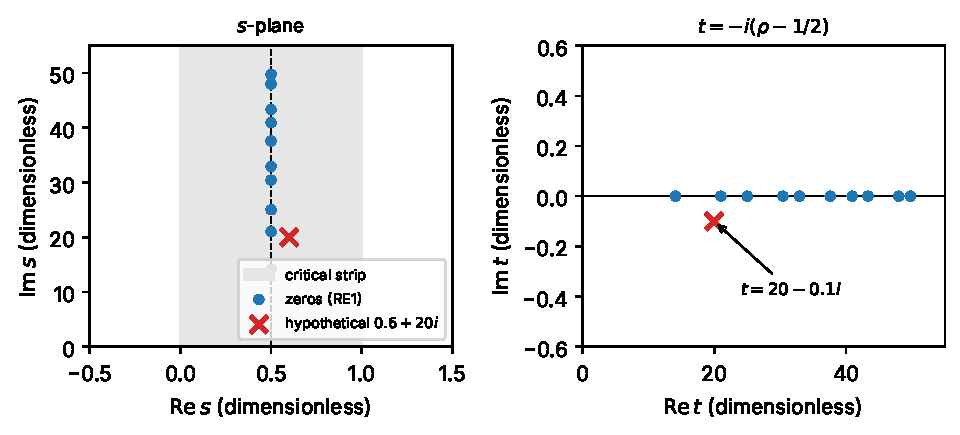
\includegraphics[width=0.85\linewidth]{figs/hilbert-polya_map.pdf}
\caption{Left: the complex $s$-plane near the critical strip $0<\Re s<1$ (shaded), with the first ten nontrivial zeros on the critical line $\Re s=\tfrac12$ (dashed) and a hypothetical zero at $0.6+20i$ off the line (cross; no such zero exists at this height). Right: the same points after the relabeling $t=-i(\rho-\tfrac12)$ of Eq.~\eqref{eq:hilbert-polya-tdef}. Zeros on the line land on the real $t$ axis; the hypothetical off-line zero lands at $t=20-0.1i$, below the axis. Both axes are dimensionless.}
\label{fig:hilbert-polya-map}
\end{figure}

\begin{sample}{Relabeling a zero}
(a) Find $t$ for the first zero $\rho_1=\tfrac12+14.134725\,i$. (b) Find $t$ for a hypothetical zero at $\rho=0.6+20i$, and say how far it would sit from the real $t$ axis.

\textbf{Step 1:} For (a), $\rho_1-\tfrac12=14.134725\,i$. Multiply by $-i$: $t=-i\cdot 14.134725\,i=14.134725\,(-i^2)=14.134725$. The value is real, as Eq.~\eqref{eq:hilbert-polya-equiv} predicts for a zero with $\sigma=\tfrac12$.

\textbf{Step 2:} For (b), $\sigma=0.6$ and $\tau=20$. Eq.~\eqref{eq:hilbert-polya-tcomplex} gives $t=20-i(0.6-0.5)=20-0.1i$.

\textbf{Step 3:} The distance from the real axis is $\abs{\Im t}=\abs{\tfrac12-\sigma}=0.1$.
\[
\boxed{t_1=14.134725,\qquad t=20-0.1i\ \ (\text{distance }0.1\text{ from the real axis})}
\]
\end{sample}

\paragraph{The symmetry of the $t$ values.} Chapter~\ref{ch:zeta} showed that nontrivial zeros come in symmetric sets: if $\rho$ is a zero, so are $1-\rho$ and the complex conjugate $\bar\rho$. Let us see what this does to $t$. For $1-\rho$:
\begin{equation}
t(1-\rho)=-i\left(1-\rho-\tfrac12\right)=-i\left(\tfrac12-\rho\right)=+i\left(\rho-\tfrac12\right)=-t(\rho).
\end{equation}
For $\bar\rho=\sigma-i\tau$, Eq.~\eqref{eq:hilbert-polya-tcomplex} with $\tau\to-\tau$ gives $t(\bar\rho)=-\tau-i(\sigma-\tfrac12)$, which is $-\overline{t(\rho)}$, because $\overline{t(\rho)}=\tau+i(\sigma-\tfrac12)$. So the full set of $t$ values is symmetric under $t\to-t$ and under $t\to\bar t$. On the critical line this just says that the zeros come in pairs $\pm t_n$. An operator that wants to have ``the zeros'' as its spectrum must therefore either have the symmetric spectrum $\{\pm t_n\}$ or be designed for the positive heights only; both choices appear in the literature.

\subsection{The conjecture}

\medskip\noindent\textbf{Conjecture (Hilbert--P\'olya; open).} There exists a self-adjoint operator $H$, acting on some space of functions, whose eigenvalues are exactly the numbers $t$ of Eq.~\eqref{eq:hilbert-polya-tdef}, one for each nontrivial zero of $\zeta$, counted with multiplicity.

\emph{Status:} conjecture. No such operator is known. Neither Hilbert nor P\'olya published the idea; it is known through later recollections, and its history and the many attempts to realize it are reviewed in \cite{schumayer}. The statement is also deliberately vague about \emph{which} space of functions and \emph{which} operator: making it precise is part of the problem.
\medskip

Why would such an operator prove RH? The argument has two links.

\textbf{Link 1: self-adjoint operators have real eigenvalues.} You met this in Chapter~\ref{ch:eigen} for matrices and in Chapter~\ref{ch:schrodinger} for operators. Here is the matrix version again, line by line. Let $H$ be a Hermitian matrix, meaning $H^\dagger=H$, where $\dagger$ is the conjugate transpose. Let $v\neq0$ be an eigenvector, $Hv=\lambda v$. Multiply on the left by $v^\dagger$:
\begin{equation}
v^\dagger H v=\lambda\, v^\dagger v .
\label{eq:hilbert-polya-real1}
\end{equation}
The number $v^\dagger v=\sum_j\abs{v_j}^2$ is real and positive because $v\ne0$. The number $q=v^\dagger Hv$ is a $1\times1$ matrix, that is, a single number. Transposing a $1\times1$ matrix does nothing, so its conjugate transpose $q^\dagger$ is just its complex conjugate $\bar q$. Therefore:
\begin{equation}
\bar q=q^\dagger=(v^\dagger Hv)^\dagger=v^\dagger H^\dagger (v^\dagger)^\dagger=v^\dagger H^\dagger v=v^\dagger Hv=q,
\label{eq:hilbert-polya-real2}
\end{equation}
using $(ABC)^\dagger=C^\dagger B^\dagger A^\dagger$ and $H^\dagger=H$. So $q$ is real, and $\lambda=q/(v^\dagger v)$ is a real number divided by a positive real number: real.

\textbf{Link 2: real $t$ means the zero is on the line.} This is Eq.~\eqref{eq:hilbert-polya-equiv}.

Chaining the links: if every $t$ is an eigenvalue of a self-adjoint $H$, every $t$ is real, so every nontrivial zero has $\sigma=\tfrac12$, which is RH. Notice what the argument needs and what it does not. It needs the operator to be self-adjoint \emph{and} needs a proof that its eigenvalues are \emph{all} the $t$ values. It does not need any particular physical interpretation; and strictly, the conclusion only uses the reality of the eigenvalues, so any operator with a proven real spectrum equal to the set of $t$'s would do. Self-adjointness is simply the most familiar guarantee of reality.

\begin{sample}{Real eigenvalues from Hermiticity, and their absence without it}
(a) Find the eigenvalues of the Hermitian matrix $H=\begin{pmatrix}2&1-i\\1+i&3\end{pmatrix}$. (b) Find the eigenvalues of the non-Hermitian matrix $B=\begin{pmatrix}1&2\\-1&1\end{pmatrix}$.

\textbf{Step 1:} Check Hermiticity of $H$. The conjugate transpose swaps the off-diagonal entries and conjugates them: the $(1,2)$ entry of $H^\dagger$ is $\overline{1+i}=1-i$, equal to $H_{12}$. The diagonal entries are real. So $H^\dagger=H$.

\textbf{Step 2:} The characteristic polynomial of a $2\times2$ matrix is $\lambda^2-(\text{trace})\lambda+\det=0$ (Chapter~\ref{ch:eigen}). Here the trace is $2+3=5$ and $\det H=2\cdot3-(1-i)(1+i)=6-(1-i^2)=6-2=4$.

\textbf{Step 3:} Solve $\lambda^2-5\lambda+4=0$: $\lambda=\tfrac12\left(5\pm\sqrt{25-16}\right)=\tfrac12(5\pm3)$, so $\lambda=1$ or $4$. Both real.

\textbf{Step 4:} For $B$, the trace is $2$ and $\det B=1\cdot1-2\cdot(-1)=3$. Solve $\lambda^2-2\lambda+3=0$: $\lambda=1\pm\sqrt{1-3}=1\pm i\sqrt2$. Complex. $B$ is real but not symmetric ($B_{12}=2\ne B_{21}=-1$), so Link 1 does not apply.
\[
\boxed{H:\ \lambda=1,\,4\qquad B:\ \lambda=1\pm i\sqrt2}
\]
\end{sample}

\begin{checkpoint}
Does a matrix need to be Hermitian in order to have only real eigenvalues? Think of the upper-triangular matrix $\begin{pmatrix}1&1\\0&2\end{pmatrix}$.
\end{checkpoint}
\checkanswer{No. That matrix is not Hermitian (its $(1,2)$ and $(2,1)$ entries are $1$ and $0$), yet its characteristic polynomial is $(1-\lambda)(2-\lambda)-1\cdot0=(1-\lambda)(2-\lambda)$, with roots $1$ and $2$, both real. Hermiticity is sufficient for real eigenvalues, not necessary. This is why some operator proposals (Section~\ref{sec:hilbert-polya-proposals}) try non-Hermitian operators with other symmetries.}

\subsection{The infinite-dimensional subtlety}

For matrices, Link 1 is airtight. For differential operators acting on functions, the analogue of ``$H^\dagger=H$'' involves integration by parts, and integration by parts produces boundary terms. Whether the boundary terms vanish depends on which functions you allow. Here is the cleanest example of what can go wrong.

\begin{sample}{A Hermitian-looking operator with complex eigenvalues}
Consider the momentum operator $\hat p=-i\,\dd/\dd x$ (units $\hbar=1$) acting on functions on the half-line $x\ge0$. (a) Show that $f(x)=e^{ikx}$ with $k=2+i$ satisfies $\hat pf=kf$ and is normalizable. (b) Show where the usual argument for real eigenvalues breaks.

\textbf{Step 1:} Differentiate: $\dd f/\dd x=ik\,e^{ikx}$, so $\hat p f=-i\cdot ik\,e^{ikx}=k\,e^{ikx}=kf$. The eigenvalue is $k=2+i$, which is complex.

\textbf{Step 2:} Normalizability: $\abs{e^{ikx}}^2=\abs{e^{i(2+i)x}}^2=\abs{e^{2ix}}^2\,\abs{e^{-x}}^2=1\cdot e^{-2x}$. So $\int_0^\infty\abs{f}^2\dd x=\int_0^\infty e^{-2x}\dd x=\tfrac12$, finite.

\textbf{Step 3:} The ``Hermiticity'' of $\hat p$ means $\int_0^\infty \bar g\,(\hat pf)\,\dd x=\int_0^\infty\overline{(\hat pg)}\,f\,\dd x$. Integrate the left side by parts:
\begin{align*}
\int_0^\infty \bar g\,(-i f')\,\dd x
&=-i\bigl[\bar g f\bigr]_0^\infty+i\int_0^\infty \bar g'\,f\,\dd x\\
&=i\,\bar g(0)f(0)+\int_0^\infty\overline{(-ig')}\,f\,\dd x ,
\end{align*}
where we used that $f,g\to0$ at infinity and $\overline{-ig'}=i\bar g'$. The extra term $i\bar g(0)f(0)$ vanishes only if $f(0)=0$ or $g(0)=0$.

\textbf{Step 4:} Our eigenfunction has $f(0)=1\neq0$, so for it the boundary term does not vanish, the operator is not symmetric on the space containing $f$, and Link 1 fails.
\[
\boxed{\text{eigenvalue }2+i,\ \ \int_0^\infty\abs f^2\dd x=\tfrac12,\ \text{broken by the boundary term } i\bar g(0)f(0)}
\]
\end{sample}

\begin{beyond}
\textbf{Symmetric versus self-adjoint.} In infinite dimensions mathematicians distinguish a \emph{symmetric} operator (the integration-by-parts identity holds for a chosen class of nice functions) from a \emph{self-adjoint} one (it is symmetric \emph{and} its domain is exactly as large as the domain of its adjoint, so no eigenfunctions can escape through boundary terms). Only self-adjoint operators come with the full guarantee that their spectrum is real. The precise definitions belong to functional analysis and are beyond this book. What matters here: any operator proposed for the Hilbert--P\'olya program must come with a proof of self-adjointness (or some other proof of reality) on a specified domain, and proposals are often most delicate exactly at this point. Half-line operators such as $\hat p$ above are relevant because the $xp$ models of Section~\ref{sec:hilbert-polya-xp} live naturally on $x>0$; see \cite{sierra} and \cite{schumayer} for discussions of these domain questions.
\end{beyond}

\subsection{What else the operator must do}

Suppose you were designing the operator. Besides self-adjointness, the facts collected in earlier chapters impose requirements. These are \emph{heuristic} design targets, discussed in \cite{berrykeating99} and reviewed in \cite{schumayer}, not theorems.

\begin{enumerate}
\item \textbf{The right average density.} The number of eigenvalues below $E$ must grow like $\Nsm(E)=\frac{E}{2\pi}\log\frac{E}{2\pi}-\frac{E}{2\pi}+\frac78$ (paper Eq.~(1), Chapter~\ref{ch:counting-zeros}). This is unusual: a particle in a box has $N(E)\propto\sqrt E$, an oscillator has $N(E)\propto E$; the zeros grow like $E\log E$.
\item \textbf{The right fluctuations.} The deviation of the true count from $\Nsm$ must reproduce the prime-power oscillations of the explicit formula (Chapter~\ref{ch:explicit-formula}). Section~\ref{sec:hilbert-polya-trace} develops what this suggests.
\item \textbf{The right statistics.} Unfolded spacings are observed numerically to follow GUE statistics closely (a numerical observation, supported by Montgomery's partial theoretical result; Chapter~\ref{ch:level-statistics}; paper Fig.~2). In random-matrix theory, complex Hermitian matrices (GUE) model systems \emph{without} time-reversal symmetry, while real symmetric matrices (GOE) model systems \emph{with} it. If the zeros are the spectrum of a chaotic quantum system, the heuristic reading is that its Hamiltonian is not time-reversal invariant.
\end{enumerate}

\paragraph{Time reversal, concretely.} Run a film of a classical motion backward: each position is unchanged, each velocity (hence momentum) is reversed. So time reversal acts as $x\to x$, $p\to-p$. A classical Hamiltonian $H(x,p)$ is time-reversal invariant if $H(x,-p)=H(x,p)$. For $H=p^2+V(x)$ (our units, $2m=1$) this holds, because $(-p)^2=p^2$. In quantum mechanics, for a particle without spin, time reversal acts on wavefunctions by complex conjugation, $\psi\to\bar\psi$. Here is why conjugation is the right operation. The plane wave $e^{ikx}$ has momentum $p=k$. Its conjugate $e^{-ikx}$ has momentum $-k$, so conjugation reverses the momentum. More generally, $\hat p=-i\,\dd/\dd x$ contains an explicit $i$. Therefore $\overline{\hat p\psi}=\overline{-i\psi'}=i\bar\psi'=-\hat p\bar\psi$, while multiplication by $x$ is unchanged by conjugation. Conjugation thus keeps $x$ and flips $p$, exactly as the backward film does. If $V$ is real, then $H=-\dd^2/\dd x^2+V$ has real coefficients, and taking the complex conjugate of $H\psi=E\psi$ (with $E$ real) gives $H\bar\psi=E\bar\psi$: the conjugate of a solution is again a solution. In matrix form, a real potential on a grid gives a real symmetric matrix (Chapter~\ref{ch:eigen}), the GOE symmetry class.

\begin{pitfall}
Do not conclude from item 3 that ``the zeros are not the spectrum of any real potential.'' The random-matrix heuristic is about \emph{generic chaotic} systems. A one-dimensional system $p^2+V(x)$ is not chaotic at all (Section~\ref{sec:hilbert-polya-trace}), so the heuristic simply does not apply to it, and, as the next Sample Problem shows, any finite list of real numbers can be the spectrum of a real symmetric matrix. Statistics constrain natural operators, not fitted ones.
\end{pitfall}

\subsection{The trap of finite lists}

There is a trivial way to ``realize'' any finite list of zeros as a spectrum, and understanding why it is trivial is the key to the last section of this chapter and to the whole paper.

\begin{sample}{An operator for two zeros}
Construct a $2\times2$ real symmetric matrix, not diagonal, whose eigenvalues are $t_1=14.134725$ and $t_2=21.022040$ (RE1). Use a rotation by $\theta=30^\circ$.

\textbf{Step 1:} Start from the diagonal matrix $D=\mathrm{diag}(t_1,t_2)$; its eigenvalues are $t_1,t_2$ with eigenvectors along the axes.

\textbf{Step 2:} Let $R=\begin{pmatrix}c&-s\\s&c\end{pmatrix}$ with $c=\cos30^\circ=\sqrt3/2$, $s=\sin30^\circ=\tfrac12$. $R$ is orthogonal, $R^\top R=I$. Set $H=RDR^\top$. If $De=\lambda e$ then $H(Re)=RDR^\top Re=RDe=\lambda Re$, so $H$ has the same eigenvalues. Also $H^\top=(R^\top)^\top D^\top R^\top=RDR^\top=H$, so $H$ is symmetric.

\textbf{Step 3:} Multiply out. $(RDR^\top)_{ij}=\sum_k R_{ik}d_kR_{jk}$, so
\begin{align*}
H_{11}&=c^2t_1+s^2t_2=0.75(14.134725)+0.25(21.022040)=15.856554,\\
H_{22}&=s^2t_1+c^2t_2=0.25(14.134725)+0.75(21.022040)=19.300211,\\
H_{12}&=cs\,t_1+(-s)c\,t_2=cs(t_1-t_2)=0.4330127\times(-6.887315)=-2.982295 .
\end{align*}

\textbf{Step 4:} Check: trace $=35.156765=t_1+t_2$, as it must be.
\[
\boxed{H=\begin{pmatrix}15.856554&-2.982295\\-2.982295&19.300211\end{pmatrix}}
\]
\end{sample}

The same recipe works for $10^4$ zeros: a diagonal $10^4\times10^4$ matrix, rotated by any orthogonal matrix you like. Such a matrix is ``a self-adjoint operator whose spectrum is the first $10^4$ zeros.'' It proves nothing, predicts nothing about zero $10^4+1$, and contains no information that was not typed into it. The Hilbert--P\'olya conjecture has content only because it asks for an operator that is \emph{specified independently of the zeros} (by geometry, by the primes, by a physical model) and whose spectrum can then be \emph{proved} to be all of them.

\begin{checkpoint}
A colleague announces a real symmetric $1000\times1000$ matrix whose eigenvalues agree with $t_1,\dots,t_{1000}$ to twelve digits. Is this evidence for RH, or for the existence of a Hilbert--P\'olya operator?
\end{checkpoint}
\checkanswer{Neither, on its own. The diagonal matrix $\mathrm{diag}(t_1,\dots,t_{1000})$ already does this, and every rotation of it does too. Agreement with data that were used to build the matrix shows only that the construction can represent that data. What would count is a prediction: an operator fixed without looking at the zeros, or at least one that predicts zeros it was not built from.}

\begin{keyideas}
\item Relabel each nontrivial zero by $t=-i(\rho-\tfrac12)$; then $\Im t=\tfrac12-\Re\rho$, so RH is the statement that every $t$ is real (Eq.~\eqref{eq:hilbert-polya-equiv}).
\item Hilbert--P\'olya conjecture (open): the $t$'s are the eigenvalues of a self-adjoint operator. With a proof that the spectrum is exactly the $t$'s, real eigenvalues would give RH.
\item In infinite dimensions, ``looks Hermitian'' is not enough; boundary terms can produce complex eigenvalues. Self-adjointness on a specified domain is required.
\item Heuristic design targets: counting function $\Nsm$, prime-power fluctuations, GUE statistics (suggesting no time-reversal symmetry).
\item Any finite list of reals is the spectrum of some symmetric matrix; reproducing finitely many zeros is not evidence by itself.
\end{keyideas}

%======================================================================
\section{Counting quantum states with classical phase space}\label{sec:hilbert-polya-phase}
%======================================================================

To compare operators with the zeros we need a quick way to estimate how many eigenvalues an operator has below an energy $E$. Physics offers a beautiful one: count area in classical phase space. Chapter~\ref{ch:wkb} develops a refined version (Bohr--Sommerfeld quantization with its $\tfrac12$); here we need only the leading rule, which we derive from the particle in a box.

\subsection{Phase space and Hamilton's equations}

The \emph{phase space} of a particle on a line is the plane with coordinates $(x,p)$: position horizontally, momentum vertically. A state of classical motion is a point; as time runs, the point moves along a curve. For a conserved energy the curve is a level curve $H(x,p)=E$ of the Hamiltonian, the energy written as a function of $x$ and $p$.

The motion along the curve is given by \emph{Hamilton's equations}. We need a \emph{partial derivative}: $\partial H/\partial p$ means ``differentiate $H$ with respect to $p$ while holding $x$ fixed,'' and similarly for $\partial H/\partial x$. Hamilton's equations are
\begin{equation}
\frac{\dd x}{\dd \tau}=\frac{\partial H}{\partial p},\qquad \frac{\dd p}{\dd \tau}=-\frac{\partial H}{\partial x}.
\label{eq:hilbert-polya-hamilton}
\end{equation}
(Here $\tau$ is time. We write $\tau$ rather than $t$ because in this book $t$ is reserved for the height of a zero; the $\tau=\Im\rho$ of Section~\ref{sec:hilbert-polya-conjecture} does not appear again, so from here on $\tau$ always means time.) Check that these reproduce Newton for $H=p^2/(2m)+V(x)$: the first gives $\dd x/\dd \tau=p/m$, the definition of momentum; the second gives $\dd p/\dd \tau=-\dd V/\dd x$, which is Newton's second law with force $-\dd V/\dd x$. In the paper's units $2m=1$, $H=p^2+V$ and $\dd x/\dd \tau=2p$.

\subsection{One state per area $2\pi\hbar$}

Take a box of length $\ell$ with hard walls. Standing waves (Chapter~\ref{ch:schrodinger}, and standing waves on a string from first-year physics) fit an integer number of half-wavelengths: $\ell=k\lambda/2$, $k=1,2,3,\dots$ By de Broglie, $p=h/\lambda=2\pi\hbar/\lambda$ (recall $\hbar=h/2\pi$), so the allowed momenta are
\begin{equation}
p_k=\frac{2\pi\hbar}{\lambda_k}=\frac{2\pi\hbar\,k}{2\ell}=\frac{\pi\hbar k}{\ell}.
\end{equation}
The number of states with momentum magnitude at most $P$ is the number of positive integers $k$ with $\pi\hbar k/\ell\le P$, i.e. the integer part of $P\ell/(\pi\hbar)$.

Now compute the phase-space area of the classical region with the same energy bound: $0\le x\le\ell$ and $-P\le p\le P$ (a classical particle bounces, so both signs of $p$ occur). It is a rectangle of area $\ell\cdot2P$. Divide by $2\pi\hbar$:
\begin{equation}
\frac{2P\ell}{2\pi\hbar}=\frac{P\ell}{\pi\hbar},
\end{equation}
exactly the count, up to rounding down. The box is a motivating example only; extending the rule to other Hamiltonians is a heuristic generalization, whose status is stated in the box below. The semiclassical counting rule reads:
\begin{equation}
N(E)\approx\frac{\text{area of }\{(x,p):H(x,p)\le E\}}{2\pi\hbar}.
\label{eq:hilbert-polya-weyl}
\end{equation}

\begin{beyond}
\textbf{Status of Eq.~\eqref{eq:hilbert-polya-weyl}.} We derived it for the box; for a general smooth one-dimensional potential it is the leading term of the WKB counting function of Chapter~\ref{ch:wkb}, valid for large $N$ with an error of order one level (the $\tfrac12$ in Bohr--Sommerfeld is part of that error). In higher dimensions the analogous statement, with $(2\pi\hbar)^d$, is Weyl's law; its proof is beyond this book. For our purposes the rule is a \emph{heuristic} that is accurate to leading order at high energy.
\end{beyond}

From now on $\hbar=1$, so each state occupies area $2\pi$. (The area rule needs only $\hbar=1$, which the paper's units $\hbar=2m=1$ include. The paper's second convention, $2m=1$, is a separate matter: it makes $H=p^2+V$, which changes the shape of the region $H\le E$ but not the rule ``area divided by $2\pi$.'')

\begin{sample}{Counting states in the paper's box}
Use RE3: an infinite well on $[-L,L]$ with $L=44.883$, in units $\hbar=2m=1$, so $E=p^2$. Estimate the number of states with $E\le1000$ by Eq.~\eqref{eq:hilbert-polya-weyl}, and compare with the exact count from $E_k=(k\pi/2L)^2$ (the squares of the allowed momenta $p_k=\pi k/\ell$ derived above, with $\ell=2L$ and $\hbar=1$).

\textbf{Step 1:} With $E=p^2$, the bound $E\le1000$ means $\abs p\le P=\sqrt{1000}=31.6228$.

\textbf{Step 2:} The region is $-L\le x\le L$, $\abs p\le P$: area $=2L\cdot2P=4LP$. Divide by $2\pi$: $N\approx 2LP/\pi=89.766\times31.6228/\pi=903.57$.

\textbf{Step 3:} Exact count: $E_k\le1000$ means $k\pi/(2L)\le\sqrt{1000}$, i.e. $k\le 2L\sqrt{1000}/\pi=903.57$. So $k=1,\dots,903$.
\[
\boxed{N_{\rm rule}\approx903.57,\qquad N_{\rm exact}=903}
\]
For comparison, when the Wu--Sprung potential is placed in this same box, it pushes the levels up and only about $650$ remain below $1000$: the paper reports 652 basis states with $E\le1000$ for its discretized smooth potential (Sec.~II~E). That potential was built so that its semiclassical count follows $\Nsm(E)$ (Chapter~\ref{ch:wu-sprung}); the value $\Nsm(1000)\approx648.62$ is computed in a Sample Problem of Section~\ref{sec:hilbert-polya-xp}. The difference of about three levels between 652 and $\Nsm(1000)$ is plausibly mainly a discretization effect. The 652 states are eigenvalues of a finite-difference matrix, and finite-difference levels lie below the continuum ones by an amount that grows with level index (Chapter~\ref{ch:finite-differences}). The paper reports that on its working grid this dispersion already reaches about two mean spacings at levels 401--500 (Sec.~II~C). The paper's Richardson-extrapolated levels, by contrast, match the smooth zeros to within $0.063$ spacings (Sec.~II~B).
\end{sample}

\begin{checkpoint}
A classical region of phase space has area $20\pi$ (units $\hbar=1$). About how many quantum states does it hold?
\end{checkpoint}
\checkanswer{About $20\pi/(2\pi)=10$.}

\subsection{Area, period and density of levels}

Two facts about closed orbits will be used repeatedly. Let $A(E)$ be the phase-space area enclosed by the closed orbit $H=E$, and $T_\gamma(E)$ its period (the subscript $\gamma$ labels the orbit; do not confuse it with the paper's training window $T$).

\textbf{Fact 1: $\dd A/\dd E=T_\gamma$.} For $H=p^2+V(x)$ with turning points $x_1<x_2$ (where $V=E$, as on any potential-energy curve), the orbit is the curve $p=\pm\sqrt{E-V(x)}$, so
\begin{equation}
A(E)=2\int_{x_1(E)}^{x_2(E)}\sqrt{E-V(x)}\,\dd x .
\end{equation}
Differentiate with respect to $E$. Both the limits and the integrand depend on $E$, so we need the rule for differentiating such an integral (the Leibniz rule):
\begin{equation}
\frac{\dd}{\dd E}\int_{a(E)}^{b(E)}g(x,E)\,\dd x=g(b,E)\,b'(E)-g(a,E)\,a'(E)+\int_{a}^{b}\frac{\partial g}{\partial E}\,\dd x .
\label{eq:hilbert-polya-leibniz}
\end{equation}
Here is where it comes from. Write $F(a,b,E)=\int_a^b g(x,E)\,\dd x$.
\begin{itemize}
\item By the fundamental theorem of calculus, $\partial F/\partial b=g(b,E)$ and $\partial F/\partial a=-g(a,E)$.
\item Differentiating under the integral sign gives $\partial F/\partial E=\int_a^b(\partial g/\partial E)\,\dd x$. We take this step on trust; it holds for the integrands met here and is stated in \cite{rhb}.
\item The chain rule for $F(a(E),b(E),E)$ adds the three contributions, which gives Eq.~\eqref{eq:hilbert-polya-leibniz}.
\end{itemize}
Apply the rule with $g=\sqrt{E-V(x)}$, $a=x_1(E)$ and $b=x_2(E)$. The integrand vanishes at both limits ($V=E$ there), so the two boundary terms are zero and only the derivative of the integrand survives:
\begin{equation}
\frac{\dd A}{\dd E}=2\int_{x_1}^{x_2}\frac{1}{2\sqrt{E-V(x)}}\,\dd x=\int_{x_1}^{x_2}\frac{\dd x}{\sqrt{E-V(x)}} .
\end{equation}
(The integrand blows up at the turning points like $1/\sqrt{\text{distance}}$, which is integrable.) The speed is $\dd x/\dd \tau=2p=2\sqrt{E-V}$ from Eq.~\eqref{eq:hilbert-polya-hamilton}, so the time to go from $x_1$ to $x_2$ is $\int\dd x/(2\sqrt{E-V})$, and the period (there and back) is twice that, $\int\dd x/\sqrt{E-V}$. Hence $\dd A/\dd E=T_\gamma(E)$.

\textbf{Fact 2: the mean level density is $T_\gamma/2\pi$.} Differentiate Eq.~\eqref{eq:hilbert-polya-weyl}: $\dd N/\dd E\approx(\dd A/\dd E)/(2\pi)=T_\gamma(E)/2\pi$. The mean spacing between levels is the reciprocal, $2\pi/T_\gamma$. In words: slow classical orbits mean densely packed quantum levels.

The \emph{action} of a closed orbit is $S_\gamma(E)=\oint p\,\dd x$, which for a one-dimensional orbit is exactly the enclosed area $A(E)$. Fact 1 therefore also says $\dd S_\gamma/\dd E=T_\gamma$. A consequence we will need: \emph{if the period is independent of energy, then $S_\gamma(E)=ET_\gamma$ up to a constant.}

\begin{keyideas}
\item Phase space is the $(x,p)$ plane; motion follows Hamilton's equations \eqref{eq:hilbert-polya-hamilton}.
\item Semiclassical rule (heuristic, leading order): one quantum state per phase-space area $2\pi\hbar$, Eq.~\eqref{eq:hilbert-polya-weyl}.
\item For a closed orbit, $\dd A/\dd E=\dd S/\dd E=T_\gamma$, so the mean level density is $T_\gamma/2\pi$.
\end{keyideas}

%======================================================================
\section{Trace formulas: periodic orbits and primes}\label{sec:hilbert-polya-trace}
%======================================================================

The most compelling reason physicists take the Hilbert--P\'olya idea seriously is a resemblance of \emph{formulas}. In quantum chaos, the fluctuating part of the level count is a sum over classical periodic orbits. In number theory, the fluctuating part of the zero count is a sum over primes. Let us build up to this comparison with an example you can check completely.

\subsection{A trace formula you can verify: equally spaced levels}

Take the equally spaced spectrum $E_k=k-\tfrac12$, $k=1,2,3,\dots$ This is the harmonic-oscillator spectrum $(k-\tfrac12)\hbar\omega$ in units where $\hbar\omega=1$. We quote these levels; they are derived in Chapter~\ref{ch:bound-states}. Nothing below depends on that derivation, since the trace formula is worked out for the list $E_k=k-\tfrac12$ itself. Its counting function $N(E)$, the number of levels with $E_k\le E$, is a staircase that jumps by 1 at $E=\tfrac12,\tfrac32,\tfrac52,\dots$ For $E\ge0$, $N(E)=\lfloor E+\tfrac12\rfloor$, where $\lfloor y\rfloor$ is the integer part (``floor'') of $y$.

We now write this staircase as ``smooth part plus oscillations,'' exactly as $N(t)=\Nsm(t)+S(t)$ in Chapter~\ref{ch:counting-zeros}. Write $\{y\}=y-\lfloor y\rfloor$ for the fractional part. Then $\lfloor y\rfloor=y-\{y\}=y-\tfrac12-\left(\{y\}-\tfrac12\right)$. The function $f(y)=\{y\}-\tfrac12$ is the sawtooth, periodic with period 1. Its Fourier series (Chapter~\ref{ch:fourier-series}) on $0<y<1$ has coefficients
\begin{align}
a_r&=2\int_0^1\left(y-\tfrac12\right)\cos(2\pi ry)\,\dd y,\qquad b_r=2\int_0^1\left(y-\tfrac12\right)\sin(2\pi ry)\,\dd y,
\end{align}
for $r\ge1$ (the Fourier coefficients for a function of period 1, Chapter~\ref{ch:fourier-series}), and $a_0=0$ because $\int_0^1(y-\tfrac12)\dd y=0$. For $b_r$, the constant $\tfrac12$ integrates to zero against a full period of the sine, and integration by parts gives
\begin{equation}
\int_0^1 y\sin(2\pi ry)\,\dd y=\left[-\frac{y\cos(2\pi ry)}{2\pi r}\right]_0^1+\int_0^1\frac{\cos(2\pi ry)}{2\pi r}\,\dd y=-\frac{1}{2\pi r}+0,
\end{equation}
so $b_r=-1/(\pi r)$. For $a_r$, integration by parts gives $\left[(y-\tfrac12)\sin(2\pi ry)/(2\pi r)\right]_0^1-\int_0^1\sin(2\pi ry)\dd y/(2\pi r)=0-0$, so $a_r=0$ for all $r\ge1$.

\begin{beyond}
The sawtooth jumps at every integer. We take on trust Dirichlet's theorem (stated in \cite{rhb}; the proof is found in standard texts on Fourier analysis): the Fourier series of a piecewise-smooth periodic function converges to the function at every point where the function is continuous, and to the midpoint of the jump at a discontinuity, with the Gibbs overshoot nearby (Chapter~\ref{ch:fourier-series}).
\end{beyond}
Hence, at every non-integer $y$,
\begin{equation}
\{y\}-\tfrac12=-\frac1\pi\sum_{r=1}^\infty\frac{\sin(2\pi ry)}{r}.
\label{eq:hilbert-polya-sawtooth}
\end{equation}
Put $y=E+\tfrac12$. Using $\sin(2\pi r E+\pi r)=(-1)^r\sin(2\pi rE)$,
\begin{align}
N(E)=\lfloor E+\tfrac12\rfloor
&=E+\tfrac12-\tfrac12+\frac1\pi\sum_{r=1}^\infty\frac{\sin\bigl(2\pi r(E+\tfrac12)\bigr)}{r}\notag\\
&=\underbrace{E}_{\text{smooth}}+\underbrace{\frac1\pi\sum_{r=1}^\infty\frac{(-1)^r}{r}\sin(2\pi rE)}_{\text{oscillating}} .
\label{eq:hilbert-polya-osctrace}
\end{align}
This is an exact \emph{trace formula} for this spectrum, valid at every $E$ that is not a level. Now interpret it classically. In units $\hbar=2m=1$, an oscillator with $\hbar\omega=1$ has Hamiltonian $H=p^2+\omega^2x^2/4$ with $\omega=1$, that is $H=p^2+x^2/4$. Its orbit at energy $E$ is an ellipse of area $A=2\pi E/\omega=2\pi E$ (Problem~19 derives this for general $\omega$). So:
\begin{itemize}
\item the smooth part $E=A/2\pi$ is the phase-space count of Eq.~\eqref{eq:hilbert-polya-weyl};
\item each oscillating term has phase $r\cdot2\pi E=rS_\gamma(E)$, where $S_\gamma=A$ is the action of the periodic orbit and $r=1,2,3,\dots$ counts how many times the orbit is traversed (its \emph{repetitions});
\item the amplitude is $1/r$, and the factor $(-1)^r$ is a phase shift of $\pi$ per traversal. We derived it from the shift $y=E+\tfrac12$ inside the floor function; that it agrees with a phase loss of $\pi/2$ at each of the two turning points (Chapter~\ref{ch:wkb}) is a consistency remark, not a separate derivation.
\end{itemize}
The discrete levels are encoded in a single periodic orbit and its repetitions. \Cref{fig:hilbert-polya-oscillator} shows the truncated sums building up the staircase.

\begin{figure}[htbp]\centering
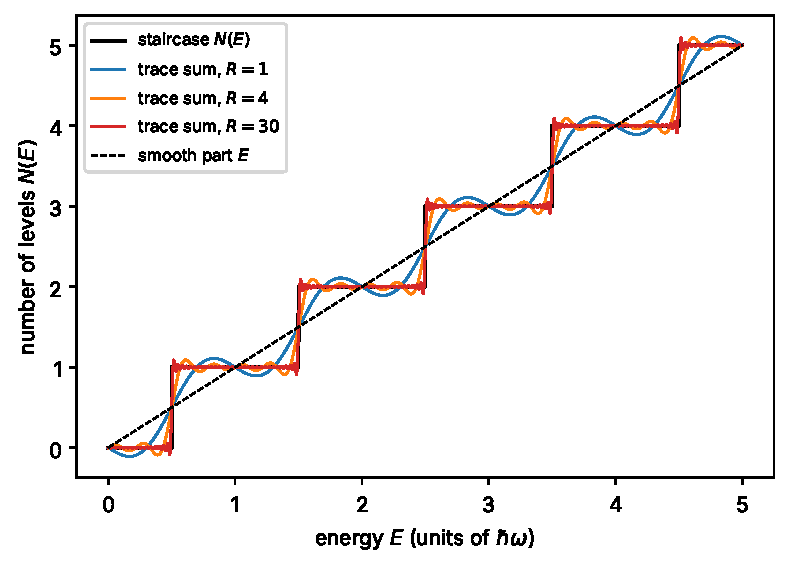
\includegraphics[width=0.85\linewidth]{figs/hilbert-polya_oscillator.pdf}
\caption{The level staircase $N(E)=\lfloor E+\tfrac12\rfloor$ of the equally spaced spectrum $E_k=k-\tfrac12$ (black), and the trace formula \eqref{eq:hilbert-polya-osctrace} truncated after $R=1$, $4$ and $30$ repetitions of the single periodic orbit. With one term the sum is a smooth wave; with more terms it sharpens into steps at the levels. Energy in units of $\hbar\omega$.}
\label{fig:hilbert-polya-oscillator}
\end{figure}

\begin{sample}{Summing the orbit series at $E=9/4$}
Evaluate the oscillating sum of Eq.~\eqref{eq:hilbert-polya-osctrace} at $E=\tfrac94$, show that it gives $N=2$ exactly, and give the partial sums through $r=1,3,5$.

\textbf{Step 1:} The levels below $\tfrac94$ are $\tfrac12$ and $\tfrac32$, so the answer should be $N=2$.

\textbf{Step 2:} The phase is $2\pi r\cdot\tfrac94=\tfrac{9\pi r}{2}$. For even $r$ this is a multiple of $\pi$ (since $9r/2$ is then an integer), so $\sin=0$.

\textbf{Step 3:} For odd $r=2j+1$ ($j=0,1,2,\dots$): $\tfrac{9\pi(2j+1)}{2}=9\pi j+\tfrac{9\pi}{2}=9\pi j+4\pi+\tfrac\pi2$. Removing $4\pi$, $\sin(9\pi j+\tfrac\pi2)=\cos(9\pi j)=(-1)^{9j}=(-1)^j$. With $(-1)^r=-1$ for odd $r$, the term is $-(-1)^j/(2j+1)$.

\textbf{Step 4:} The sum is $-\left(1-\tfrac13+\tfrac15-\tfrac17+\cdots\right)$. The bracket is the Leibniz series. It converges, because it is alternating with terms decreasing to zero (Chapter~\ref{ch:series}). To find its value, start from the geometric series (Chapter~\ref{ch:series}) with ratio $-u^2$: for $\abs u<1$, $\frac{1}{1+u^2}=1-u^2+u^4-u^6+\cdots$. Integrate both sides from $0$ to $x$, with $\abs x<1$. The left side gives $\arctan x$, because $\frac{\dd}{\dd x}\arctan x=\frac{1}{1+x^2}$ and $\arctan0=0$; the right side, integrated term by term, gives
\[
\arctan x=x-\frac{x^3}{3}+\frac{x^5}{5}-\frac{x^7}{7}+\cdots\qquad(\abs x<1).
\]
At $x=1$ the series becomes the Leibniz bracket, and $\arctan 1=\pi/4$.
\begin{beyond}
Two steps are taken on trust here: integrating a power series term by term inside its interval of convergence, and passing to the endpoint $x=1$, where the series still converges (Abel's theorem: if a power series converges at an endpoint of its interval, its sum there is the limit of the function). Abel's theorem and term-by-term integration are stated in \cite{rhb}; proofs are in standard real-analysis texts. Numerically, two million terms of the Leibniz series agree with $\pi/4=0.785398$ to six decimal places.
\end{beyond}
So
\[
N\!\left(\tfrac94\right)=\tfrac94+\frac1\pi\left(-\frac\pi4\right)=\tfrac94-\tfrac14=2 .
\]

\textbf{Step 5:} Partial sums: through $r=1$, $\tfrac94-\tfrac1\pi=1.931690$; through $r=3$, add $\tfrac{1}{3\pi}=0.106103$ to get $2.037793$; through $r=5$, subtract $\tfrac1{5\pi}=0.063662$ to get $1.974131$.
\[
\boxed{N(9/4)=2;\quad \text{partial sums }1.931690,\ 2.037793,\ 1.974131}
\]
The partial sums oscillate around 2 and approach it slowly. Orbit sums of this kind converge only conditionally, if at all; this echoes the convergence issues you met in Chapter~\ref{ch:explicit-formula}.
\end{sample}

\subsection{Gutzwiller's trace formula}

For a chaotic system there is no single orbit family; at each energy there are infinitely many isolated periodic orbits, each unstable. Gutzwiller found the analogous formula for chaotic systems. It has the same structure (a smooth term plus a sum over orbits and their repetitions), but it is asymptotic rather than exact. Each orbit also carries a stability factor that has no counterpart in Eq.~\eqref{eq:hilbert-polya-osctrace}.

\begin{beyond}
\textbf{Gutzwiller's trace formula} (an asymptotic approximation for small $\hbar$, derived by the stationary-phase method; derivation beyond this book, see \cite{gutzwiller}). For a quantum system with two degrees of freedom (for example a particle moving in a plane, so that phase space is four-dimensional) whose classical limit is chaotic with isolated unstable periodic orbits, the level count is approximately
\begin{equation}
N(E)\approx\bar N(E)+\frac1\pi\sum_{\gamma}\sum_{r=1}^\infty\frac{1}{r}\,\frac{\sin\!\bigl(rS_\gamma(E)/\hbar-r\mu_\gamma\pi/2\bigr)}{\abs{\det\left(M_\gamma^r-I\right)}^{1/2}} .
\label{eq:hilbert-polya-gutz}
\end{equation}
Here $\bar N$ is the smooth phase-space count; $\gamma$ runs over \emph{primitive} periodic orbits (orbits traversed once), $r$ over repetitions; $S_\gamma$ is the action; $\mu_\gamma$ is an integer (the Maslov index) counting turning-point-like phase losses; and $M_\gamma$ is the \emph{stability matrix}, the $2\times2$ matrix (for a two-dimensional system) that maps a small displacement away from the orbit, measured across the orbit, to its value one period later. The formula is usually written for the level density $\dd N/\dd E$, whose oscillating terms are $\frac{1}{\pi\hbar}\,T_\gamma\cos\bigl(rS_\gamma/\hbar-r\mu_\gamma\pi/2\bigr)/\abs{\det(M_\gamma^r-I)}^{1/2}$. To pass to the count, integrate in $E$. By the chain rule and $\dd S_\gamma/\dd E=T_\gamma$ (we derived this relation only for one-dimensional motion; it holds for periodic orbits in general, which we take on trust, see \cite{gutzwiller}), $\frac{\dd}{\dd E}\sin\bigl(rS_\gamma/\hbar-r\mu_\gamma\pi/2\bigr)=\frac{rT_\gamma}{\hbar}\cos\bigl(rS_\gamma/\hbar-r\mu_\gamma\pi/2\bigr)$. Treating $T_\gamma$ and the determinant as constant over one oscillation (this is the approximation: their slow energy dependence is neglected), $\int T_\gamma\cos(\cdots)\,\dd E\approx\frac{\hbar}{r}\sin(\cdots)$, so the prefactor becomes $\frac{1}{\pi\hbar}\cdot\frac{\hbar}{r}=\frac{1}{\pi r}$, which is the form above. For chaotic systems the orbit sum does not converge absolutely; it is meaningful as an asymptotic statement and after smoothing.
\end{beyond}

\paragraph{The stability factor of an unstable orbit.} For an unstable (hyperbolic) orbit, a small displacement grows by a factor $\Lambda=e^{\lambda T_\gamma}>1$ per period along one direction and shrinks by $1/\Lambda$ along another; $\lambda$ is the Lyapunov exponent (the growth rate). This $\lambda$ is neither the eigenvalue $\lambda$ of Section~\ref{sec:hilbert-polya-conjecture} nor the wavelength $\lambda$ of the box count in Section~\ref{sec:hilbert-polya-phase}. The stability matrix then has eigenvalues $\Lambda$ and $1/\Lambda$. (This $\Lambda$ is a growth factor; it has nothing to do with the von Mangoldt function $\Lambda(k)$ of Chapter~\ref{ch:primes}.)
\begin{beyond}
That the two eigenvalues multiply to 1, i.e. $\det M_\gamma=1$, follows from the fact that Hamiltonian motion preserves phase-space area (Liouville's theorem). We take this on trust; see \cite{gutzwiller}.
\end{beyond}
After $r$ traversals the eigenvalues of $M^r_\gamma$ are $\Lambda^r$ and $\Lambda^{-r}$. For any $2\times2$ matrix $B$ with eigenvalues $\beta_1,\beta_2$, the characteristic polynomial is $\det(B-zI)=(\beta_1-z)(\beta_2-z)$. Both sides are quadratics in $z$ with leading coefficient $1$ and roots $\beta_1,\beta_2$, so they are equal. Putting $z=1$,
\begin{align}
\det\left(M_\gamma^r-I\right)&=(\Lambda^r-1)(\Lambda^{-r}-1)\notag\\
&=\Lambda^r\Lambda^{-r}-\Lambda^r-\Lambda^{-r}+1\notag\\
&=2-\Lambda^r-\Lambda^{-r}=-\left(\Lambda^{r/2}-\Lambda^{-r/2}\right)^2 ,
\end{align}
where the last step expands $(\Lambda^{r/2}-\Lambda^{-r/2})^2=\Lambda^r-2+\Lambda^{-r}$. Therefore
\begin{equation}
\abs{\det\left(M_\gamma^r-I\right)}^{1/2}=\Lambda^{r/2}-\Lambda^{-r/2}=e^{r\lambda T_\gamma/2}-e^{-r\lambda T_\gamma/2}\approx e^{r\lambda T_\gamma/2}\quad\text{(for }r\lambda T_\gamma\gg1).
\label{eq:hilbert-polya-stab}
\end{equation}
Unstable orbits are exponentially suppressed in the sum: the more unstable, the weaker their contribution.

\subsection{The explicit formula as a trace formula}

Now put the zeros' version next to it. From Chapter~\ref{ch:explicit-formula}, the fluctuating part of $N(t)$ is approximated (heuristically; the series does not converge on the critical line, and the truncation is an approximation whose accuracy is measured numerically) by paper Eq.~(4):
\begin{equation}
N(t)\approx\Nsm(t)+\Nfl(t),\qquad
\Nfl(t)=-\frac1\pi\sum_{p\in P}\sum_{m=1}^{3}\frac{\sin(mt\log p)}{m\,p^{m/2}} ,
\label{eq:hilbert-polya-nfl}
\end{equation}
with $P$ a finite set of primes. The comparison with Gutzwiller's formula below concerns the untruncated formal sum $-\frac1\pi\sum_{p}\sum_{m=1}^{\infty}\sin(mt\log p)/(m\,p^{m/2})$, taken over all primes and all $m$. Eq.~\eqref{eq:hilbert-polya-nfl} is a truncation of that sum. Term by term the two are the same, so the dictionary can be read off from either. Read Eqs.~\eqref{eq:hilbert-polya-gutz} and \eqref{eq:hilbert-polya-nfl} side by side, with energy $E\leftrightarrow$ height $t$ and $\hbar=1$. (The comparison is with Gutzwiller's formula for a hypothetical chaotic system with two degrees of freedom, whose stability matrices are $2\times2$; each prime is treated as a primitive orbit of such a system. It is not a comparison with a one-dimensional potential, which is not chaotic.)
\begin{itemize}
\item Both have the form ``smooth part $+\frac1\pi\sum_{\text{primitive}}\sum_{\text{repetitions}}\frac1{\text{rep.}}\times\frac{\text{oscillation}}{\text{stability}}$.''
\item The phase $mt\log p$ matches $rS_\gamma(E)$ if each prime $p$ is a primitive orbit with $S_p(E)=E\log p$, and $m$ is the repetition number. By Fact 1 of Section~\ref{sec:hilbert-polya-phase} ($T=\dd S/\dd E$), $S_p(E)=E\log p$ gives $T_p=\log p$, a period independent of energy.
\item The amplitude $p^{-m/2}$ matches $e^{-r\lambda T_\gamma/2}$ (the large-$r\lambda T$ form of Eq.~\eqref{eq:hilbert-polya-stab}) if $T_\gamma=\log p$ and $\lambda=1$: then $e^{m\log p/2}=p^{m/2}$. Every ``prime orbit'' would have the same Lyapunov exponent, 1.
\item The smooth part $\Nsm$ would be the phase-space count $\bar N$.
\end{itemize}
\Cref{tab:hilbert-polya-dictionary} collects this dictionary.

\begin{table}[htbp]\centering
\caption{The trace-formula dictionary between a chaotic quantum system (Gutzwiller, Eq.~\eqref{eq:hilbert-polya-gutz}) and the Riemann zeros (explicit formula, Eq.~\eqref{eq:hilbert-polya-nfl}). This is an \emph{analogy}: no dynamical system with these properties is known. The last two rows are where the analogy is imperfect.}
\label{tab:hilbert-polya-dictionary}
\begin{tabular}{ll}
\toprule
chaotic system & Riemann zeros\\
\midrule
energy $E$ & height $t$\\
smooth count $\bar N(E)$ & $\Nsm(t)$, paper Eq.~(1)\\
primitive periodic orbit $\gamma$ & prime $p$\\
period $T_\gamma$ & $\log p$\\
repetition number $r$ & power $m$ (prime power $p^m$)\\
action $rS_\gamma(E)=rET_\gamma$ & $mt\log p$\\
stability $\abs{\det(M^r-I)}^{1/2}$ & $p^{m/2}$ (matches only for large $p^m$, with $\lambda=1$)\\
phase $-r\mu_\gamma\pi/2$ & overall minus sign (not of Maslov form)\\
\bottomrule
\end{tabular}
\end{table}

\begin{figure}[htbp]\centering
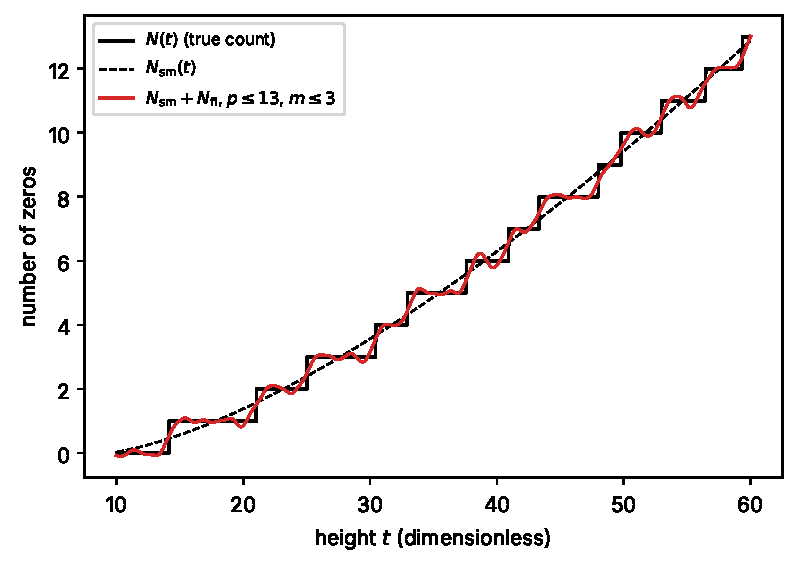
\includegraphics[width=0.85\linewidth]{figs/hilbert-polya_zetastair.pdf}
\caption{The zero-counting staircase $N(t)$ for $10\le t\le60$ (black; it jumps by 1 at each zero $t_n$ of RE1 and beyond), the smooth count $\Nsm(t)$ of paper Eq.~(1) (dashed), and $\Nsm(t)+\Nfl(t)$ with the six primes $p\le13$ and $m\le3$ (paper Eq.~(4), solid color). The ``prime-orbit'' sum bends the smooth curve toward the steps. Height $t$ is dimensionless.}
\label{fig:hilbert-polya-zetastair}
\end{figure}

\begin{sample}{The $p=2$ orbit}
In the dictionary, find the period, the frequency in $t$, the period in $t$, and the counting-function amplitude of the $p=2$, $m=1$ term (RE2). Then compare its stability factor with the exact hyperbolic value of Eq.~\eqref{eq:hilbert-polya-stab}.

\textbf{Step 1:} Period $T_2=\log2=0.693147$. The term $\sin(t\log2)$ oscillates in $t$ with angular frequency $\log 2$, hence with period in $t$ equal to $2\pi/\log2=9.064720$, the RE2 value.

\textbf{Step 2:} Amplitude in $\Nfl$: $\frac1\pi\cdot\frac{1}{1\cdot2^{1/2}}=\frac{1}{\pi\sqrt2}=0.225079$. So this single term moves the count up and down by about $0.23$ of a zero.

\textbf{Step 3:} The explicit formula's stability factor is $2^{1/2}=1.414214$. The exact hyperbolic factor with $\Lambda=e^{\lambda T}=e^{\log2}=2$ is $\Lambda^{1/2}-\Lambda^{-1/2}=1.414214-0.707107=0.707107$.

\textbf{Step 4:} Ratio: $1.414214/0.707107=2$. In general the ratio is $p^{m/2}/(p^{m/2}-p^{-m/2})=1/(1-p^{-m})$, which is $2$ for $p^m=2$ and tends to 1 for large $p^m$.
\[
\boxed{T_2=0.693147,\ \ 2\pi/\log2=9.064720,\ \ \text{amplitude }0.225079,\ \ \text{stability ratio }2}
\]
\end{sample}

\subsection{Where the analogy is imperfect}

An honest dictionary records its failures. Three stand out.

\textbf{The sign.} Eq.~\eqref{eq:hilbert-polya-nfl} has an overall minus sign for \emph{every} $p$ and $m$. In Eq.~\eqref{eq:hilbert-polya-gutz} the corresponding quantity is the phase shift $-r\mu_\gamma\pi/2$ inside the sine. Since $\sin(\theta-\phi)=\sin\theta\cos\phi-\cos\theta\sin\phi$ equals $-\sin\theta$ for all $\theta$ exactly when $\cos\phi=-1$ and $\sin\phi=0$, that is, when $\phi\equiv\pi\pmod{2\pi}$, a constant sign $-1$ needs $r\mu\pi/2\equiv\pi\pmod{2\pi}$ for every $r$. For $r=1$ this means $\mu\pi/2\equiv\pi$, so $\mu\equiv2\pmod4$. For $r=2$ it means $\mu\pi\equiv\pi$, so $\mu$ is odd. These two conditions contradict each other (Problem~10). This mismatch is discussed in the literature; Connes interprets the zeros as an \emph{absorption} spectrum (lines missing from a continuum) rather than as emitted eigenvalues \cite{connes}.

\textbf{The stability factor.} As the Sample Problem showed, $p^{m/2}$ is only the large-$p^m$ limit of the hyperbolic factor; for $p=2$, $m=1$ they differ by a factor 2. The naive dictionary works asymptotically, not exactly.

\textbf{No dynamics.} Nobody has exhibited a classical system whose primitive periodic orbits have periods $\log 2,\log 3,\log 5,\dots$, all with Lyapunov exponent 1. The dictionary is a description of what such a system would have to look like.

\begin{checkpoint}
In the dictionary, which ``orbit'' does the term $\sin(2t\log 3)/(2\cdot3)$ of $\Nfl$ correspond to, and what is its total traversal time?
\end{checkpoint}
\checkanswer{The primitive orbit $p=3$ traversed $m=2$ times (the prime power $9$). Its primitive period is $\log3$, so two traversals take $2\log3=\log9\approx2.197$. The amplitude $1/(2\cdot3)$ is $1/(m p^{m/2})$ with $p^{m/2}=3$.}

\begin{figure}[htbp]\centering
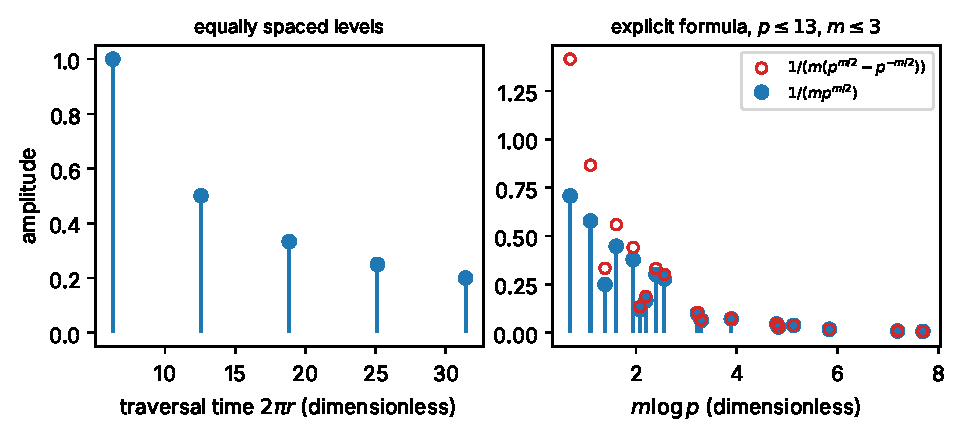
\includegraphics[width=0.85\linewidth]{figs/hilbert-polya_orbits.pdf}
\caption{``Orbit spectra'': the amplitude of each oscillating term in a trace formula, plotted at its action per unit energy (that is, at its total traversal time, the angular frequency of the term in $E$ or $t$). Left: the equally spaced spectrum of Eq.~\eqref{eq:hilbert-polya-osctrace}, one orbit of period $2\pi$ and its repetitions, amplitudes $1/r$. Right: the explicit formula, Eq.~\eqref{eq:hilbert-polya-nfl}, with $p\le13$, $m\le3$: stems at $m\log p$ with heights $1/(mp^{m/2})$; open circles show the heights $1/\bigl(m(p^{m/2}-p^{-m/2})\bigr)$ that an exactly hyperbolic orbit with $\lambda=1$ would give. The overall factor $1/\pi$ and the signs are omitted. Horizontal axes are dimensionless.}
\label{fig:hilbert-polya-orbits}
\end{figure}

\subsection{A heuristic consequence for one-dimensional potentials}

Here is an observation, \emph{heuristic} and clearly labeled, that becomes important in the paper. A one-dimensional potential $p^2+V(x)$ has, at each energy, exactly one periodic orbit: the back-and-forth motion between the two turning points. Its trace formula is therefore of the oscillator type, Eq.~\eqref{eq:hilbert-polya-osctrace}, with $2\pi E$ replaced by the action $S(E)=A(E)$: a single orbit and its repetitions. Those terms produce the steps of the staircase; they do not produce independent oscillations at frequencies $\log2,\log3,\dots$ in $E$. So a one-dimensional potential can only reproduce the zeros' fluctuations by building them into the \emph{shape} of $V$, so that the phase-space area $A(E)/2\pi$ itself contains $\Nsm(E)+\Nfl(E)$. This is the spirit of what Wu and Sprung did (Chapter~\ref{ch:wu-sprung}): a smooth potential from $\Nsm$, plus fitted fluctuating corrections that make the levels reproduce the low zeros. In such a construction the fluctuations sit in the shape of the potential as fine wiggles; they are not generated dynamically. The fluctuation at energy $E$ is then controlled by the potential near the turning points of that energy, that is, locally in energy. We will meet this picture again in the paper's Sec.~VI.

\begin{keyideas}
\item A trace formula writes the level count as a smooth phase-space term plus a sum over periodic orbits and their repetitions; Eq.~\eqref{eq:hilbert-polya-osctrace} is an exact, checkable example.
\item Gutzwiller's formula \eqref{eq:hilbert-polya-gutz} (asymptotic; proof beyond this book) weights unstable orbits by $1/\abs{\det(M^r-I)}^{1/2}\approx e^{-r\lambda T/2}$.
\item The explicit formula \eqref{eq:hilbert-polya-nfl} has the same shape with primes as primitive orbits, periods $\log p$, repetitions $m$, and stability $p^{m/2}$ (Table~\ref{tab:hilbert-polya-dictionary}). This is an analogy, not a theorem.
\item The analogy is imperfect: an overall minus sign not of Maslov form, $p^{m/2}$ matching the hyperbolic factor only for large $p^m$, and no known dynamics.
\item Heuristically, a 1D potential has one orbit per energy and can carry prime oscillations only in its shape.
\end{keyideas}

%======================================================================
\section{The Berry--Keating Hamiltonian \texorpdfstring{$H=xp$}{H = xp}}\label{sec:hilbert-polya-xp}
%======================================================================

The dictionary asks for unstable orbits, all with Lyapunov exponent 1, and no time-reversal symmetry. Berry and Keating \cite{berrykeating99} noticed that the simplest conceivable Hamiltonian has all three features:
\begin{equation}
H(x,p)=xp .
\label{eq:hilbert-polya-xp}
\end{equation}

\subsection{Classical motion}

Hamilton's equations \eqref{eq:hilbert-polya-hamilton} with $H=xp$: $\partial H/\partial p=x$ and $\partial H/\partial x=p$, so
\begin{equation}
\frac{\dd x}{\dd \tau}=x,\qquad\frac{\dd p}{\dd \tau}=-p .
\end{equation}
These are the growth and decay equations of first-year physics, with solutions $x(\tau)=x_0e^{\tau}$ and $p(\tau)=p_0e^{-\tau}$ ($\tau$ is time, as in Section~\ref{sec:hilbert-polya-phase}). Their product $x(\tau)p(\tau)=x_0p_0$ is constant: energy is conserved and the orbits are hyperbolas $xp=E$ (\cref{fig:hilbert-polya-xp}). Every orbit stretches $x$ by $e^\tau$ and squeezes $p$ by $e^{-\tau}$ in time $\tau$: a small displacement grows at rate $\lambda=1$, the same for every orbit. That is the exponent the dictionary wants.

Time reversal sends $p\to-p$: $H(x,-p)=-xp\ne H(x,p)$. So $xp$ is \emph{not} time-reversal invariant, consistent with the GUE heuristic of Section~\ref{sec:hilbert-polya-conjecture}.

The trouble is equally visible: the hyperbolas are not closed. A particle runs off to $x\to\infty$ and never returns. There are no periodic orbits at all, and the phase-space region $xp\le E$ has infinite area.

\begin{figure}[htbp]\centering
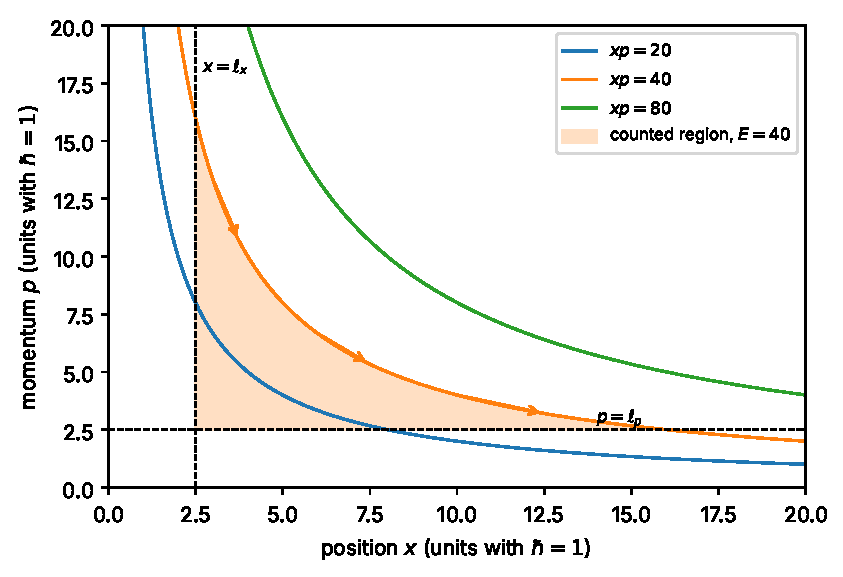
\includegraphics[width=0.85\linewidth]{figs/hilbert-polya_xp.pdf}
\caption{Phase space of $H=xp$ in the quadrant $x>0$, $p>0$ (units $\hbar=1$). Orbits are hyperbolas $xp=E$ (curves for $E=20,40,80$), traversed in the direction of the arrows ($x$ grows, $p$ shrinks). The Berry--Keating regularization keeps only $x\ge\ell_x$ and $p\ge\ell_p$ with $\ell_x\ell_p=2\pi$ (dashed lines, drawn with $\ell_x=\ell_p=\sqrt{2\pi}$); the shaded region is the part of $xp\le40$ that is counted. Its area divided by $2\pi$ gives Eq.~\eqref{eq:hilbert-polya-nbk}.}
\label{fig:hilbert-polya-xp}
\end{figure}

\subsection{Regularizing and counting}

Berry and Keating cut phase space off by hand: keep only $x\ge\ell_x$ and $p\ge\ell_p$ for two positive constants, and count the region of the quadrant $x>0$, $p>0$ with $xp\le E$ (\cref{fig:hilbert-polya-xp}). For the region to be non-empty we need $E>\ell_x\ell_p$. At a given $x$, the allowed $p$ run from $\ell_p$ up to $E/x$; the largest $x$ is where these meet, $x=E/\ell_p$. So
\begin{align}
A(E)&=\int_{\ell_x}^{E/\ell_p}\left(\frac Ex-\ell_p\right)\dd x\notag\\
&=E\bigl[\log x\bigr]_{\ell_x}^{E/\ell_p}-\ell_p\left(\frac{E}{\ell_p}-\ell_x\right)\notag\\
&=E\log\frac{E}{\ell_x\ell_p}-E+\ell_x\ell_p .
\label{eq:hilbert-polya-area}
\end{align}
The cutoffs enter only through their product $a=\ell_x\ell_p$, a phase-space area. Berry and Keating chose $a=2\pi\hbar=2\pi$, one Planck cell. The motivation is the counting rule itself: a quantum state occupies an area $2\pi\hbar$, so phase-space structure on a smaller area cannot be resolved, and a cutoff of one cell is the natural minimal choice. (Problem~7 shows that any other choice adds a term growing like $E$ and spoils the agreement below). With $a=2\pi$ and the counting rule \eqref{eq:hilbert-polya-weyl}:
\begin{equation}
N_{\rm BK}(E)=\frac{A(E)}{2\pi}=\frac{E}{2\pi}\log\frac{E}{2\pi}-\frac{E}{2\pi}+1 .
\label{eq:hilbert-polya-nbk}
\end{equation}
Compare with paper Eq.~(1): $\Nsm(t)=\frac{t}{2\pi}\log\frac{t}{2\pi}-\frac{t}{2\pi}+\frac78$. The two growing terms agree exactly; the constants differ:
\begin{equation}
N_{\rm BK}(E)-\Nsm(E)=1-\tfrac78=\tfrac18 .
\label{eq:hilbert-polya-eighth}
\end{equation}
A crude classical count with one Planck-cell cutoff reproduces the leading asymptotics of the zero count, the $E\log E$ growth that no box or oscillator produces. Be careful about what is independent here. The coefficient $\frac{1}{2\pi}$ of $E\log E$ does not depend on the cutoff area $a$ (Problem~7), so it is a genuine output of the $xp$ dynamics. The linear term $-\frac{E}{2\pi}$ matches only because $a=2\pi$ was chosen, so that agreement is a consistency check of the choice, not independent evidence. This is why $xp$ is regarded as a suggestive starting point, not as a solution. The difference of $\tfrac18$ of a level is well within the order-one error of the counting rule itself, so the computation says nothing about the constant.

\begin{sample}{The Berry--Keating count at $E=1000$}
Evaluate $\Nsm(1000)$ and $N_{\rm BK}(1000)$, and compare with the true number of zeros up to height 1000.

\textbf{Step 1:} $1000/(2\pi)=159.15494$ and $\log159.15494=5.069878$.

\textbf{Step 2:} The growing part: $159.15494\times(5.069878-1)=159.15494\times4.069878=647.7412$.

\textbf{Step 3:} $\Nsm(1000)=647.7412+0.875=648.6162$ and $N_{\rm BK}(1000)=647.7412+1=648.7412$.

\textbf{Step 4:} Counting the zeros (with \texttt{qmnt.zeros}; see the listing that follows this Sample Problem) gives $N(1000)=649$: the 649th zero lies below $1000$ and the 650th above. The fluctuating part at this height is $N(1000)-\Nsm(1000)\approx0.38$.
\[
\boxed{\Nsm(1000)\approx648.62,\quad N_{\rm BK}(1000)\approx648.74,\quad N(1000)=649}
\]
\end{sample}

\begin{pycode}
import numpy as np, qmnt
t = qmnt.zeros(700)                    # t_1 ... t_700 (t_700 > 1000)
def Nsm(E):  return E/(2*np.pi)*np.log(E/(2*np.pi)) - E/(2*np.pi) + 7/8
def NBK(E):  return Nsm(E) + 1/8       # Eq. (hilbert-polya-nbk)
for E in [100.0, 500.0, 1000.0]:
    N = np.sum(t <= E)                  # true count N(E)
    print(E, N, round(Nsm(E), 3), round(NBK(E), 3))
# last line printed: 1000.0 649 648.616 648.741
\end{pycode}

\subsection{The orbit time and the level density}

Fact 2 of Section~\ref{sec:hilbert-polya-phase} says the mean level density is (orbit time)$/2\pi$. Does it hold for the regularized $xp$? The orbit enters the counted region at $x=\ell_x$ and leaves at $x=E/\ell_p$. Since $x=x_0e^\tau$, the time spent inside is $T(E)$ (a transit time; again not the paper's training window $T$) with $e^{T}=(E/\ell_p)/\ell_x$:
\begin{equation}
T(E)=\log\frac{E}{\ell_x\ell_p}=\log\frac{E}{2\pi}.
\end{equation}
Meanwhile, differentiating Eq.~\eqref{eq:hilbert-polya-area} with $\ell_x\ell_p=2\pi$,
\begin{equation}
\frac{\dd A}{\dd E}=\log\frac{E}{2\pi}+E\cdot\frac1E-1=\log\frac{E}{2\pi}=T(E),
\end{equation}
in agreement with Fact 1. Note that here $T(E)$ is a \emph{transit time} between the two cutoffs, not the period of a closed orbit (the hyperbolas never close); the relation $\dd A/\dd E=T$ is verified directly by the two computations just made. The density $\dd N_{\rm BK}/\dd E=\frac{1}{2\pi}\log\frac{E}{2\pi}$ is the mean density of the zeros, and its reciprocal $2\pi/\log(E/2\pi)$ is the mean spacing of Chapter~\ref{ch:counting-zeros}, the paper's $\gap_n$ evaluated at height $E$. The zeros crowd together because the orbit time grows logarithmically.

\begin{sample}{Orbit time and spacing at $E=1000$}
Find $T(1000)$ and the mean spacing of the zeros at height $1000$.

\textbf{Step 1:} $T(1000)=\log(1000/2\pi)=\log159.15494=5.069878$.

\textbf{Step 2:} Mean spacing $=2\pi/T=6.283185/5.069878=1.239317$.
\[
\boxed{T(1000)\approx5.0699,\qquad \text{spacing}\approx1.2393}
\]
Near height 1000, consecutive zeros are about $1.24$ apart on average, compared with $t_2-t_1\approx6.9$ at the bottom.
\end{sample}

\begin{figure}[htbp]\centering
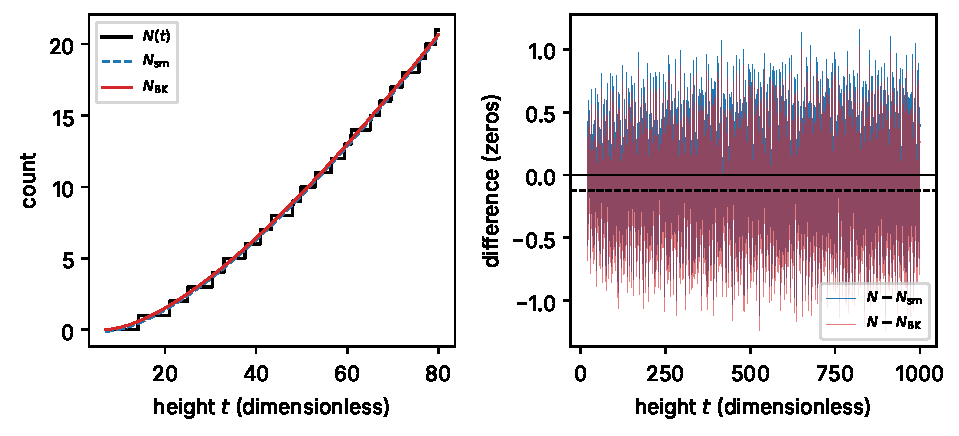
\includegraphics[width=0.85\linewidth]{figs/hilbert-polya_bk.pdf}
\caption{Left: the true count $N(t)$ (staircase), $\Nsm(t)$ of paper Eq.~(1) and the Berry--Keating count $N_{\rm BK}(t)$ of Eq.~\eqref{eq:hilbert-polya-nbk} for $0<t\le80$; the two smooth curves differ by the constant $\tfrac18$. Right: $N(t)-\Nsm(t)$ and $N(t)-N_{\rm BK}(t)$ for $20\le t\le1000$. Both fluctuate (the fluctuation is $S(t)$ of Chapter~\ref{ch:counting-zeros}), around $0$ and $-\tfrac18$ respectively; neither smooth curve drifts away from the data. All quantities dimensionless.}
\label{fig:hilbert-polya-bk}
\end{figure}

\subsection{The quantum $xp$ operator}

To make $xp$ a quantum operator we replace $p$ by $\hat p=-i\,\dd/\dd x$ (with $\hbar=1$). The classical product $xp$ does not fix the order of the quantum operators, and the order matters. From the lines below, $\hat p\hat x\psi-\hat x\hat p\psi=-i(\psi+x\psi')+ix\psi'=-i\psi$. Moreover, neither ordering alone is Hermitian. Formally, $(\hat x\hat p)^\dagger=\hat p^\dagger\hat x^\dagger=\hat p\hat x$, using $(AB)^\dagger=B^\dagger A^\dagger$ and the fact that $\hat x$ and $\hat p$ are each formally Hermitian; this differs from $\hat x\hat p$. Their average is formally Hermitian, because taking $\dagger$ just swaps its two terms. So one symmetrizes:
\begin{equation}
\hat H=\tfrac12\left(\hat x\hat p+\hat p\hat x\right).
\end{equation}
Acting on a function $\psi(x)$:
\begin{align}
\hat x\hat p\,\psi&=-ix\psi',\notag\\
\hat p\hat x\,\psi&=-i(x\psi)'=-i(\psi+x\psi'),\notag\\
\hat H\psi&=\tfrac12\left(-ix\psi'-i\psi-ix\psi'\right)=-i\left(x\psi'+\tfrac12\psi\right).
\label{eq:hilbert-polya-xpop}
\end{align}

\begin{sample}{Eigenfunctions of the quantum $xp$}
Show that $\psi_E(x)=x^{-1/2+iE}$ ($x>0$) satisfies $\hat H\psi_E=E\psi_E$ for every real $E$, and show that it is not normalizable.

\textbf{Step 1:} For complex powers use $x^a=e^{a\log x}$ (Chapter~\ref{ch:complex}); then $\frac{\dd}{\dd x}x^a=a\,x^{a-1}$ as for real $a$, since $\frac{\dd}{\dd x}e^{a\log x}=\frac ax e^{a\log x}$.

\textbf{Step 2:} With $a=-\tfrac12+iE$: $x\psi_E'=a\,x^{a}=\left(-\tfrac12+iE\right)\psi_E$.

\textbf{Step 3:} So $x\psi_E'+\tfrac12\psi_E=iE\,\psi_E$, and Eq.~\eqref{eq:hilbert-polya-xpop} gives $\hat H\psi_E=-i\cdot iE\,\psi_E=E\psi_E$.

\textbf{Step 4:} Modulus: $\abs{x^{iE}}=\abs{e^{iE\log x}}=1$, so $\abs{\psi_E}^2=x^{-1}$. Then $\int_1^X x^{-1}\dd x=\log X\to\infty$ as $X\to\infty$, and similarly $\int_\epsilon^1x^{-1}\dd x=\log(1/\epsilon)\to\infty$ as $\epsilon\to0$.
\[
\boxed{\hat H\,x^{-1/2+iE}=E\,x^{-1/2+iE}\ \text{for all real }E;\quad\int_0^\infty\abs{\psi_E}^2\dd x=\infty}
\]
\end{sample}

Every real number is a (generalized, non-normalizable) eigenvalue: the spectrum of the plain quantum $xp$ is the whole real line, continuous, like a free particle's. (In the variable $u=\log x$, $\psi_E=e^{-u/2}e^{iEu}$ is a plane wave in $u$, which explains the analogy.) The regularization that produced discrete counting in Eq.~\eqref{eq:hilbert-polya-nbk} was a classical cutoff drawn by hand, not a property of an operator. Turning those cutoffs into genuine boundary conditions or interactions that make the spectrum discrete, with the right density, and then showing that the eigenvalues are the zeros, is the unsolved part. Sierra \cite{sierra} reviews attempts along this line, including modified $xp$ Hamiltonians designed to make the orbits bounded and the spectrum discrete.

\begin{checkpoint}
Is $H=xp$ time-reversal invariant? Is $H=p^2+x^2$?
\end{checkpoint}
\checkanswer{Under $p\to-p$, $xp\to-xp$, so $xp$ is not invariant. $p^2+x^2\to(-p)^2+x^2=p^2+x^2$, so the oscillator is invariant.}

\begin{keyideas}
\item $H=xp$ has hyperbolic orbits $x\propto e^\tau$, $p\propto e^{-\tau}$ ($\tau$ = time), Lyapunov exponent 1, and broken time-reversal symmetry: the features the dictionary asks for.
\item With phase-space cutoffs $\ell_x\ell_p=2\pi$, the semiclassical count is $N_{\rm BK}=\frac{E}{2\pi}\log\frac{E}{2\pi}-\frac E{2\pi}+1$, matching $\Nsm$ except for the constant ($1$ versus $\tfrac78$), Eqs.~\eqref{eq:hilbert-polya-nbk}--\eqref{eq:hilbert-polya-eighth}.
\item The orbit time $\log(E/2\pi)$ gives the mean density of zeros.
\item The quantum $\tfrac12(\hat x\hat p+\hat p\hat x)$ has continuous spectrum (eigenfunctions $x^{-1/2+iE}$); the cutoffs are not an operator. The $xp$ idea reproduces averages, not the zeros.
\end{keyideas}

%======================================================================
\section{Other routes: Connes, Bender--Brody--M\"uller, Sierra and recent proposals}\label{sec:hilbert-polya-proposals}
%======================================================================

The analytic program has produced many candidate constructions. We describe the ones the paper cites, at the level of what they attempt and what their authors report, without verdicts beyond what is published. Throughout, keep in mind the one fact not in dispute: \emph{the Riemann hypothesis remains open}, so no construction has been accepted as a proof.

\paragraph{Connes: trace formulas in noncommutative geometry.} Connes \cite{connes} works not with a Schr\"odinger operator but with an action of the multiplicative group on a space built from all the primes at once (the ``ad\`ele class space,'' an object from number theory whose definition is beyond this book). In that setting he obtains a spectral interpretation of the critical zeros, as an \emph{absorption} spectrum (zeros appear as missing lines), and shows that RH is equivalent to the validity of a certain trace formula. That trace formula is closely related to the Weil form of the explicit formula (the duality between zeros and prime powers stated in Chapter~\ref{ch:explicit-formula}); Weil had shown that RH is equivalent to the positivity of a quadratic form built from that explicit formula, and proving such a positivity is the goal of this line of work. The paper also cites a 2026 contribution \cite{connes26}: as the paper reports (Sec.~I~A~b and Sec.~II~D), extremizing the truncated Weil quadratic form over primes $p\le13$ yields approximations to the first 50 zeros with accuracies from $10^{-3}$ down to $2.6\times10^{-55}$, provably located on the critical line. Note the logic: this uses only prime data, never a zero.

\paragraph{Zeta spectral triples.} Connes, Consani and Moscovici \cite{zetatriples} construct operators from Euler products over primes, with numerically observed spectral convergence (the paper's description, Sec.~I~A~d). Again the input is arithmetic, not zero data.

\paragraph{Bender, Brody and M\"uller.} Bender, Brody and M\"uller \cite{bbm} proposed an operator built from the symmetrized $\hat x\hat p+\hat p\hat x$ of Section~\ref{sec:hilbert-polya-xp} combined with the shift operator $e^{-i\hat p}$ (which shifts a function's argument by one unit). Its formal eigenfunctions are related to the Hurwitz zeta function, a relative of $\zeta$, and, as the authors describe, a boundary condition at $x=0$ selects eigenvalues that correspond to the zeros of $\zeta$ (see \cite{bbm} for the construction). The operator is not Hermitian in the ordinary sense; the authors argued that it has a symmetry of the kind studied by Bender and Boettcher for non-Hermitian Hamiltonians with real spectra \cite{bender98} (PT symmetry; Chapter~\ref{ch:non-hermitian}), and that if a suitable inner product can be constructed, the eigenvalues are real. Recall the Checkpoint of Section~\ref{sec:hilbert-polya-conjecture}: reality does not require ordinary Hermiticity, which is why this route is conceivable. Bellissard published a comment \cite{bellissard} disputing aspects of this argument; we do not summarize its technical content here. Whatever one's view of the exchange, RH remains open.

\paragraph{Sierra.} Sierra \cite{sierra} reviews the program of realizing the zeros as a spectrum, centered on $xp$-type Hamiltonians and their modifications, aimed at replacing the hand-drawn cutoffs of Eq.~\eqref{eq:hilbert-polya-area} by genuine quantum boundary conditions or interactions, and discusses what such constructions would and would not imply for RH.

\paragraph{Recent proposals.} Yakaboylu \cite{recenthp1} proposes a Hamiltonian intended to realize the Hilbert--P\'olya conjecture; Tamburini \cite{recenthp2} proposes a relativistic approach based on a Majorana particle in a $(1{+}1)$-dimensional Rindler spacetime. The paper cites these, with the others above, as evidence that ``explicit operator candidates continue to be proposed'' (Sec.~I). We do not assess them.

\begin{table}[htbp]\centering
\caption{Analytic operator proposals cited in the paper, by their input and their published status. ``Input'' records whether zero data are used in building the operator. None of these constructions is accepted as a proof of RH, which remains open.}
\label{tab:hilbert-polya-proposals}
\begin{tabular}{lll}
\toprule
proposal & input & what is reported\\
\midrule
Berry--Keating $xp$ \cite{berrykeating99} & classical model & leading count $\Nsm$; quantum spectrum continuous\\
Connes \cite{connes} & primes (ad\`eles) & RH equivalent to a trace formula\\
Connes 2026 \cite{connes26} & primes $p\le13$ & first 50 zeros, accuracies to $2.6\times10^{-55}$\\
Connes--Consani--Moscovici \cite{zetatriples} & Euler products & numerically observed spectral convergence\\
Bender--Brody--M\"uller \cite{bbm} & $xp$ and shift & eigenvalues tied to zeros; reality argued; disputed in \cite{bellissard}\\
Sierra \cite{sierra} & modified $xp$ & review and modified models\\
Yakaboylu \cite{recenthp1}; Tamburini \cite{recenthp2} & models & recent proposals\\
\bottomrule
\end{tabular}
\end{table}

\begin{checkpoint}
Which of the constructions in \cref{tab:hilbert-polya-proposals} use zero data as input?
\end{checkpoint}
\checkanswer{None. They are all specified from other principles (classical dynamics, primes, Euler products, symmetry), which is what makes their output a prediction rather than a fit. This is the defining feature of the analytic program.}

\begin{keyideas}
\item Connes gives a spectral (absorption) interpretation in which RH is equivalent to the validity of a trace formula. By Weil's earlier criterion, RH is also equivalent to the positivity of a quadratic form built from the explicit formula. A 2026 construction from primes $p\le13$ reproduces the first 50 zeros to very high accuracy (as reported in paper Sec.~I~A~b).
\item Bender--Brody--M\"uller propose a non-Hermitian, PT-type operator linked to the Hurwitz zeta function; Bellissard published a comment disputing aspects of the argument.
\item Sierra and others refine $xp$; new proposals continue to appear.
\item No operator is known whose spectrum is proved to be the zeros and that is proved self-adjoint (or proved to have real spectrum). RH and the Hilbert--P\'olya conjecture remain open.
\end{keyideas}

%======================================================================
\section{Two programs: analytic and empirical}\label{sec:hilbert-polya-programs}
%======================================================================

There is a second, quite different way to pursue the dream. Instead of specifying an operator and computing its spectrum, you \emph{fit} an operator to the zeros you already know. Wu and Sprung \cite{wusprung} built a smooth one-dimensional potential whose semiclassical count is $\Nsm$ (Chapter~\ref{ch:wu-sprung}) and then added fitted fluctuating corrections so that its levels reproduce the low zeros; van Zyl and Hutchinson \cite{vanzyl}, Slater \cite{slater} and Jaksch \cite{jaksch} refined such reconstructions. Call this the \emph{empirical} program.

The two programs differ in the direction of the arrow (\cref{fig:hilbert-polya-programs}):
\begin{itemize}
\item \textbf{Analytic:} principles $\to$ operator $\to$ spectrum $\to$ compare with zeros. Every agreement is a prediction, because the zeros were not used. A disagreement refutes the proposal.
\item \textbf{Empirical:} zeros $\to$ fit operator parameters $\to$ spectrum $\to$ compare with the same zeros. Agreement is guaranteed to the extent the family is flexible enough; it measures capacity.
\end{itemize}

The implicit hope of the empirical program is that a potential reproducing many zeros accurately has captured something about the putative zeta operator. The Sample Problem ``An operator for two zeros'' shows why agreement on the training data cannot by itself test that hope: a rotated diagonal matrix reproduces any finite list exactly. What \emph{can} test it is the standard question of every data-driven science: does the fitted operator predict zeros it was not shown? If it has captured structure, it should; if it has only stored the data, it should not. This is the question of memorization versus generalization (Chapter~\ref{ch:generalization}), and it is the question the paper asks.

The trace-formula picture of Section~\ref{sec:hilbert-polya-trace} also suggests, heuristically, what to expect. The structure that would transfer to unseen zeros is the prime-orbit sum: oscillations at fixed frequencies $m\log p$ in $t$ that continue forever. A one-dimensional potential addresses each level through its turning points, locally in energy, and has only one orbit per energy. A fit can bend the potential to reproduce a window of oscillations, but nothing in the parametrization says ``keep oscillating at frequency $\log2$ above the window.'' Whether this heuristic is right is an empirical question, and Part~VI shows how the paper tests it.

\begin{figure}[htbp]\centering
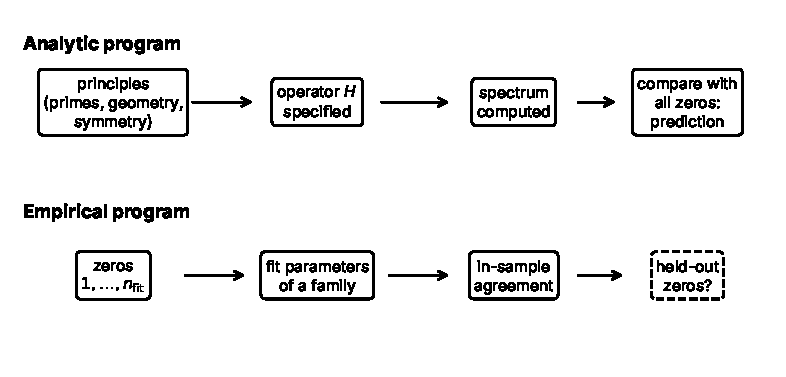
\includegraphics[width=0.85\linewidth]{figs/hilbert-polya_programs.pdf}
\caption{The two programs. Top (analytic): an operator is specified from principles that do not involve the zeros, its spectrum is computed and compared with all zeros, so every agreement is a prediction. Bottom (empirical): operator parameters are fitted to the known zeros $1,\dots,n_{\rm fit}$, and agreement on those zeros is the usual criterion of success. The dashed box is the test this program had lacked and that the paper applies: prediction of held-out zeros.}
\label{fig:hilbert-polya-programs}
\end{figure}

\begin{checkpoint}
A fitted potential reproduces zeros 1--400 to rms $0.14$ mean spacings, while predicting no fluctuation at all gives $0.24$. Does this show the potential has learned the zeros' structure?
\end{checkpoint}
\checkanswer{No. Those are in-sample numbers, and a flexible enough family can reproduce any sequence of that size. What matters is how it does on zeros it was not fitted to, compared with the null on those same zeros. (These particular numbers are the paper's: in-sample rms $0.137$ at $M=400$ and in-sample null $0.2438$, App.~A key anchors; Section~\ref{sec:hilbert-polya-paper} tells you what happened out of sample.)}

\begin{keyideas}
\item Analytic program: specify, then predict; agreement is evidence. Empirical program: fit, then compare; in-sample agreement measures capacity.
\item The decisive test for a fitted operator is held-out prediction relative to its own null.
\item Heuristically, the transferable structure is a sum of fixed-frequency oscillations in $t$, which a locally acting 1D potential has no built-in way to continue.
\end{keyideas}

%======================================================================
\section{Paper connection}\label{sec:hilbert-polya-paper}
%======================================================================

\paragraph{Sec.~I, first paragraph.} The paper opens with the conjecture in exactly the form of Section~\ref{sec:hilbert-polya-conjecture}: the $t_n$ of $\rho_n=\tfrac12+it_n$ ``are the spectrum of a self-adjoint operator.'' It then lists the circumstantial evidence in three items, each of which this chapter (with its prerequisites) unpacks:
\begin{enumerate}
\item ``Montgomery's pair-correlation theorem and Odlyzko's numerics match Gaussian unitary ensemble (GUE) eigenvalue statistics'' \cite{montgomery,odlyzko87}. This is Chapter~\ref{ch:level-statistics}, and it is the statistical design target of Section~\ref{sec:hilbert-polya-conjecture}, with its heuristic reading as broken time-reversal symmetry. The paper's Fig.~2 shows the GUE spacing histogram for the first $10^4$ zeros and uses it only to validate the dataset and unfolding (Sec.~II~A), not as evidence for any operator.
\item ``the zero-counting function resembles a semiclassical trace formula in which the primes play the role of periodic orbits'' \cite{berrykeating99,schumayer}. This is Section~\ref{sec:hilbert-polya-trace} and \cref{tab:hilbert-polya-dictionary}. The word ``resembles'' is exactly right: it is an analogy with known imperfections.
\item ``explicit operator candidates continue to be proposed'' \cite{connes,bbm,bellissard,sierra,recenthp1,recenthp2,zetatriples}. These are the seven references of Section~\ref{sec:hilbert-polya-proposals} and \cref{tab:hilbert-polya-proposals}. Note that the paper includes Bellissard's comment in the same citation list without taking sides, and so do we.
\end{enumerate}

\paragraph{Sec.~I, second paragraph and the scope statement.} ``Alongside this analytic program runs an empirical one,'' citing \cite{wusprung,vanzyl,slater,jaksch}: this is the distinction of Section~\ref{sec:hilbert-polya-programs}. The paper states the implicit logic (``a potential reproducing many zeros accurately has captured something about the putative zeta operator'') and then the scope: ``We do not test, and make no claim against, analytic Hilbert--P\'olya constructions in which an operator is specified independently of the zeros and its spectrum is then predicted.'' After this chapter you can see why the scope is natural: an analytic construction already makes predictions about every zero, so the held-out question is built into it; the fitted constructions are the ones for which in-sample agreement was the criterion. The scope is also narrower than ``all empirical constructions'': only fluctuation potentials added to the Wu--Sprung background, in three bases (cosine, Chebyshev, hat; paper Sec.~II~C), were tested.

\paragraph{Sec.~I~A~d, ``Operator proposals.''} The paper says the analytic program ``seeks exact operators and is not our target,'' singles out the zeta spectral triples \cite{zetatriples} as ``prime-driven construction, not a fit to zero data,'' and concludes: ``Our results constrain only the empirical shortcut: the hope that fitting flexible operator families to finitely many zeros captures transferable structure.'' The ``Input'' column of \cref{tab:hilbert-polya-proposals} is the criterion being used.

\paragraph{Sec.~I~A~b and Sec.~II~D: arithmetic constructions.} The paper places Connes' 2026 construction \cite{connes26} ``on the arithmetic side of our comparison,'' because it ``consumes only prime data.'' Its role in the paper is to show that ``the predictive information is arithmetic and abundantly accessible without fitting.'' The paper's own arithmetic baseline is the much simpler truncated orbit sum, paper Eq.~(4), our Eq.~\eqref{eq:hilbert-polya-nfl} with $m\le3$ and a finite prime set, which the paper calls an ``information-existence baseline'' and for which it explicitly claims no novelty. In trace-formula language, the oracle is ``the prime-orbit sum, truncated to the shortest orbits.''

\paragraph{Fig.~1 and Table~V.} Fig.~1 of the paper shows the contrast this chapter prepares you for: on zeros past the training boundary, a fitted operator (fit on zeros 1--400, scale 1, $M=400$) has held-out correlation $-0.07$, while the six-prime explicit formula, with zero fitted parameters, has $+0.96$. The six-prime row of Table~V gives rms $0.074$ and correlation $+0.96$ on zeros 401--500, against the null $0.263$ (RE5). You can reproduce that row in a few seconds:
\begin{pycode}
import numpy as np, qmnt
n    = np.arange(401, 501)                         # RE5 holdout
true = qmnt.zeros(500)[n - 1]
null = qmnt.rms(qmnt.fluct(true, n))               # predict t_n = s_n
pred = qmnt.oracle_zeros(n, qmnt.first_primes(6), mmax=3)  # p <= 13
rms, corr = qmnt.score(pred, n)
print(round(null, 4), round(rms, 3), round(corr, 2))   # 0.2631 0.074 0.96
\end{pycode}
The ``prime orbits'' $2,3,5,7,11,13$, the shortest periods in \cref{fig:hilbert-polya-orbits}, already carry most of the predictable fluctuation.

\paragraph{Sec.~VI, first and second paragraphs.} ``Nothing here touches the analytic Hilbert--P\'olya program \cite{berrykeating99,connes,bbm,zetatriples,connes26}. What is constrained is a shortcut.'' Read with this chapter, the sentence is precise: the analytic program's hard problems (self-adjointness on a domain, a proof that the spectrum is all the zeros) are untouched by any numerical fit. The second paragraph offers a \emph{heuristic} reading of why the fits fail: the fitted quantity ``is, by the explicit formula, an almost-periodic function of $t$ that is sparse in frequency, whereas a potential addresses the levels through their turning points, locally in energy.'' That is the picture of the end of Section~\ref{sec:hilbert-polya-trace} and of Section~\ref{sec:hilbert-polya-programs}: one orbit per energy in 1D, versus fixed prime-orbit frequencies in $t$. The paper is careful to call this a heuristic, to say it is ``evidence about the tested parametrizations and optimizer together, not a statement about what a potential can represent,'' and to list as open ``whether the memorization result can be derived rather than measured.'' Keep those hedges when you retell the result.

\paragraph{The falsifiability standard.} Finally, the paper's proposal (Sec.~VI, items (i)--(iv)) applies to ``any future claim that a constructed or learned operator `captures' the Riemann zeros.'' In our reading (the paper does not say this), an analytically specified operator meets the spirit of item (i) (held-out rms and correlation against its own smooth part) once its spectrum is actually computed and scored, since no zero was used to build it. The paper's list makes no exemption. For a fitted operator, item (i) is the whole question. Chapters~\ref{ch:paper-setup}--\ref{ch:paper-critique} read these items in detail.

%======================================================================
\section{Summary}
%======================================================================
\begin{itemize}
\item Relabel each nontrivial zero by $t=-i(\rho-\tfrac12)$; then $\Im t=\tfrac12-\Re\rho$ (Eq.~\eqref{eq:hilbert-polya-tcomplex}), so RH $\iff$ all $t$ real (Eq.~\eqref{eq:hilbert-polya-equiv}). The $t$ values are symmetric under $t\to-t$ and $t\to\bar t$.
\item Hilbert--P\'olya conjecture (open): the $t$ values are the eigenvalues of a self-adjoint operator. Hermitian $\Rightarrow$ real eigenvalues (Eqs.~\eqref{eq:hilbert-polya-real1}--\eqref{eq:hilbert-polya-real2}), so a proved realization would give RH. In infinite dimensions self-adjointness on a domain is essential; boundary terms can produce complex eigenvalues.
\item Any finite list of reals is the spectrum of a symmetric matrix; finite agreement is not evidence.
\item Semiclassical counting: one state per phase-space area $2\pi\hbar$ (Eq.~\eqref{eq:hilbert-polya-weyl}); $\dd A/\dd E=\dd S/\dd E=T_\gamma$; mean density $T_\gamma/2\pi$.
\item Trace formulas: exact for equally spaced levels (Eq.~\eqref{eq:hilbert-polya-osctrace}); Gutzwiller for chaotic systems (Eq.~\eqref{eq:hilbert-polya-gutz}, asymptotic), with hyperbolic stability factor $\Lambda^{r/2}-\Lambda^{-r/2}$ (Eq.~\eqref{eq:hilbert-polya-stab}).
\item The explicit formula (Eq.~\eqref{eq:hilbert-polya-nfl}, paper Eq.~(4)) resembles a trace formula with primes as orbits of period $\log p$, repetitions $m$, stability $p^{m/2}$ (Table~\ref{tab:hilbert-polya-dictionary}); the analogy fails in the sign and at small $p^m$, and no dynamics is known.
\item Berry--Keating $xp$ (Eq.~\eqref{eq:hilbert-polya-xp}): with cutoffs $\ell_x\ell_p=2\pi$, $N_{\rm BK}=\frac E{2\pi}\log\frac E{2\pi}-\frac E{2\pi}+1=\Nsm+\tfrac18$ (Eqs.~\eqref{eq:hilbert-polya-nbk}--\eqref{eq:hilbert-polya-eighth}); orbit time $\log(E/2\pi)$; the quantum operator has continuous spectrum (Eq.~\eqref{eq:hilbert-polya-xpop}).
\item Connes, Bender--Brody--M\"uller (with Bellissard's comment), Sierra, Yakaboylu, Tamburini, Connes--Consani--Moscovici: analytic proposals built without zero data; none accepted as a proof.
\item Analytic program (specify, predict) versus empirical program (fit, compare): the paper tests only the latter, by held-out prediction.
\end{itemize}

%======================================================================
\section{Problems}
%======================================================================
\begin{problemlist}
\prob{1}{Find $t=-i(\rho-\tfrac12)$ for (a) $\rho=\tfrac12+21.022040\,i$ (the second zero of RE1), and (b) the hypothetical point $\rho=0.55+30i$. For (b), give $\Im t$ and state what its sign tells you.}

\prob{1}{Show that $H=\begin{pmatrix}3&2i\\-2i&3\end{pmatrix}$ is Hermitian and find its eigenvalues.}

\prob{1}{Which of the following classical Hamiltonians are time-reversal invariant ($p\to-p$)? (a) $p^2+x^4$; (b) $xp$; (c) $x^2p^2$; (d) $p^3$.}

\prob{1}{A box of length $\ell=10$ in units $\hbar=2m=1$ has levels $E_k=(k\pi/\ell)^2$. Estimate the number of states with $E\le100$ by the area rule \eqref{eq:hilbert-polya-weyl} and compare with the exact count.}

\prob{2}{In the level density $\dd\Nfl/\dd t$, the term from prime $p$ with $m=1$ has amplitude $\frac1\pi\log p/\sqrt p$. (a) Derive this from Eq.~\eqref{eq:hilbert-polya-nfl}. (b) Compute $\log p/\sqrt p$ for $p=2,3,5,7,11,13$. (c) Show that the function $\log y/\sqrt y$ has its maximum at $y=e^2$, and say which prime gives the largest density amplitude.}

\prob{2}{Repeat the Sample Problem ``Summing the orbit series'' at $E=\tfrac74$: show that the oscillating sum of Eq.~\eqref{eq:hilbert-polya-osctrace} reduces to $+\tfrac1\pi(1-\tfrac13+\tfrac15-\cdots)$ and that $N(\tfrac74)=2$.}

\prob{2}{Redo the Berry--Keating count with a general cutoff area $a=\ell_x\ell_p$. Show that $N(E)=\frac{E}{2\pi}\log\frac{E}{2\pi}-\frac E{2\pi}+\frac{E}{2\pi}\log\frac{2\pi}{a}+\frac a{2\pi}$, and explain why only $a=2\pi$ is compatible with $\Nsm$ at large $E$.}

\prob{2}{Using $\dd N_{\rm BK}/\dd E$, compute the mean spacing of the zeros at height $t_{500}=811.1843588$ (paper App.~A key anchors). Compare with the spacing at height $1000$ found in the text.}

\prob{2}{Compute the ratio $1/(1-p^{-m})$ between the explicit formula's stability factor $p^{m/2}$ and the exact hyperbolic factor $p^{m/2}-p^{-m/2}$ for (a) $p=2$, $m=3$ and (b) $p=13$, $m=1$. Which terms of the explicit formula are best described by the hyperbolic-orbit dictionary?}

\prob{2}{Show that no integer Maslov index $\mu$ makes the phase shift $r\mu\pi/2$ congruent to $\pi$ modulo $2\pi$ (equivalently $e^{-ir\mu\pi/2}=-1$) for both $r=1$ and $r=2$. Conclude that the explicit formula's overall sign cannot be produced by the phase term of Eq.~\eqref{eq:hilbert-polya-gutz}.}

\prob{2}{(a) Verify by direct differentiation that $\psi_E(x)=x^{-1/2+iE}$ satisfies $-i(x\psi'+\psi/2)=E\psi$. (b) Compute $\int_1^{X}\abs{\psi_E}^2\dd x$ and its limit as $X\to\infty$. (c) In the variable $u=\log x$, what kind of function is $\sqrt x\,\psi_E$?}

\prob{2}{(a) Give a $2\times2$ real matrix that is not symmetric but has real eigenvalues. (b) Explain why the Hilbert--P\'olya argument needs only the reality of the eigenvalues, and why self-adjointness is nevertheless the usual requirement.}

\prob{2}{(Paper.) Read the scope statement in Sec.~I of the paper. (a) List what is tested and what is explicitly not tested. (b) Classify each of the following as analytic or empirical in the sense of Section~\ref{sec:hilbert-polya-programs}: Wu--Sprung \cite{wusprung}, van Zyl--Hutchinson \cite{vanzyl}, Slater \cite{slater}, Jaksch \cite{jaksch}, Berry--Keating \cite{berrykeating99}, Connes \cite{connes}, Bender--Brody--M\"uller \cite{bbm}, Connes--Consani--Moscovici \cite{zetatriples}.}

\prob{2}{(Paper.) Sec.~I~A~b of the paper reports accuracies from $10^{-3}$ down to $2.6\times10^{-55}$ for Connes' 2026 construction. (a) How many orders of magnitude does this range span? (b) Why does the paper say this construction ``strengthens the paper's conclusion'' rather than competing with it?}

\prob{2}{(Paper.) Using Table~V of the paper, compute the ratio (oracle rms)/(null rms) for six primes and for 25 primes on the holdouts 401--500 and 5001--10000. How do the corresponding correlations change? What reason does the table caption give for the mild growth of rms at a fixed prime budget?}

\prob{2}{(Computational, paper.) Using \texttt{qmnt}, reproduce the 3-prime and 25-prime entries of Table~V of the paper on the holdout 401--500, and check the null $0.263$.}

\prob{3}{(Computational.) Using \texttt{qmnt.zeros}, compute $D_1(T)=N(T)-\Nsm(T)$ and $D_2(T)=N(T)-N_{\rm BK}(T)$ on a fine grid of $T$ in $[100,1000]$, and their averages over the grid. Explain your results using Eq.~\eqref{eq:hilbert-polya-eighth}.}

\prob{3}{(Computational.) Using numpy, compute the partial sums of Eq.~\eqref{eq:hilbert-polya-osctrace} at $E=\tfrac94$ for $R=1,\dots,200$ repetitions. Plot the error $\abs{N_R-2}$ against $R$ and show that it stays below $1/(\pi R)$ for odd $R$. What does the slow decay say about truncating orbit sums?}

\prob{3}{For $H=p^2+\omega^2x^2/4$ (an oscillator in units $2m=1$): (a) show the orbit $H=E$ is an ellipse and compute its area $A(E)$; (b) verify $\dd A/\dd E=T_\gamma$ with $T_\gamma=2\pi/\omega$; (c) deduce from the area rule that the level spacing is $\omega$ (that is, $\hbar\omega$).}

\prob{3}{(a) For the stable orbit of a rotation, $M=\begin{pmatrix}\cos\alpha&-\sin\alpha\\\sin\alpha&\cos\alpha\end{pmatrix}$, compute $\det(M^r-I)$. (b) Contrast with the hyperbolic result \eqref{eq:hilbert-polya-stab}: which kind of orbit gives amplitudes that decay exponentially with $r$?}

\prob{2}{Construct a $3\times3$ real symmetric, non-diagonal matrix whose eigenvalues are $t_1,t_2,t_3$ of RE1, and explain in two sentences why such a matrix is no evidence for any Hilbert--P\'olya operator.}

\prob{2}{(Paper.) Explain which of the paper's criteria (i)--(iv) in Sec.~VI an analytically specified operator, such as one built from primes alone, satisfies ``automatically,'' and which it still needs to address.}

\prob{2}{(Paper.) The paper's Hermitian fitted potentials are real, so their Hamiltonians are time-reversal invariant, whereas the zeros show GUE statistics (paper Fig.~2). Explain why this does not prevent the fits from matching the training zeros closely in-sample (paper Sec.~III), and why GUE statistics alone do not single out any particular operator.}

\prob{3}{(Paper.) Using the heuristic of Section~\ref{sec:hilbert-polya-trace} (one periodic orbit per energy for a 1D potential), explain the paper's Sec.~VI reading that ``a potential addresses the levels through their turning points, locally in energy,'' and relate it to the arithmetic-continuation probe of paper Sec.~III, in which a fit to a window of the $p=2$ oscillation (RE2) did not continue it (held-out correlation $+0.07$). State clearly what is heuristic in your argument.}

\prob{1}{Label each statement as theorem (proved), numerical observation, analogy/heuristic, or open conjecture: (a) Hermitian matrices have real eigenvalues; (b) RH; (c) the Hilbert--P\'olya conjecture; (d) the unfolded spacings of the first $10^4$ zeros follow the GUE Wigner surmise closely; (e) primes are the periodic orbits of a chaotic system; (f) with cutoffs $\ell_x\ell_p=2\pi$, the classical area of $xp\le E$ divided by $2\pi$ is $\Nsm(E)+\tfrac18$.}

\prob{2}{(Computational.) Using \texttt{qmnt}, evaluate $N(t)$, $\Nsm(t)$ and $\Nsm(t)+\Nfl(t)$ (six primes, $m\le3$) at $t=100,500,1000$ and comment on how much of the fluctuation $N-\Nsm$ the six ``prime orbits'' capture at each height.}
\end{problemlist}

%======================================================================
\section{Answers to selected problems}
%======================================================================

\textbf{Problem 1.} (a) $\rho-\tfrac12=21.022040\,i$, so $t=-i\cdot21.022040\,i=21.022040$, real. (b) Eq.~\eqref{eq:hilbert-polya-tcomplex}: $t=30-i(0.55-0.5)=30-0.05i$, so $\Im t=-0.05$. The negative sign means $\sigma>\tfrac12$: the point is to the right of the critical line.

\textbf{Problem 2.} $H^\dagger$: the $(1,2)$ entry is $\overline{-2i}=2i=H_{12}$, diagonal real, so Hermitian. Trace $6$, determinant $9-(2i)(-2i)=9-4=5$. $\lambda^2-6\lambda+5=0$ gives $\lambda=1,5$.

\textbf{Problem 3.} (a) $(-p)^2+x^4$: invariant. (b) $-xp$: not invariant. (c) $x^2(-p)^2=x^2p^2$: invariant. (d) $(-p)^3=-p^3$: not invariant.

\textbf{Problem 4.} $E=p^2\le100$ means $\abs p\le10$. Area $\ell\cdot2\cdot10=200$; divided by $2\pi$: $31.83$. Exact: $k\pi/10\le10$, so $k\le100/\pi=31.83$, i.e. $31$ states.

\textbf{Problem 5.} (a) $\frac{\dd}{\dd t}\sin(t\log p)=\log p\cos(t\log p)$, so the $m=1$ term of $\dd\Nfl/\dd t$ is $-\frac1\pi\frac{\log p}{\sqrt p}\cos(t\log p)$. (b) $0.490$, $0.634$, $0.720$, $0.735$, $0.723$, $0.711$ for $p=2,3,5,7,11,13$. (c) $\frac{\dd}{\dd y}\frac{\log y}{\sqrt y}=\frac{1}{y\sqrt y}-\frac{\log y}{2y\sqrt y}=\frac{2-\log y}{2y^{3/2}}$, zero at $\log y=2$, positive below and negative above: a maximum at $y=e^2\approx7.39$. Among primes, $p=7$ gives the largest amplitude. (In the counting function itself the amplitude $1/\sqrt p$ decreases with $p$; differentiation multiplies by the frequency $\log p$.)

\textbf{Problem 7.} Eq.~\eqref{eq:hilbert-polya-area} with general $a$: $A=E\log(E/a)-E+a$. Write $\log(E/a)=\log(E/2\pi)+\log(2\pi/a)$ and divide by $2\pi$ to get the stated form. Compared with $\Nsm$, there is an extra term $\frac{E}{2\pi}\log\frac{2\pi}{a}$, which grows linearly in $E$ and would eventually exceed any constant error unless $\log(2\pi/a)=0$, i.e. $a=2\pi$.

\textbf{Problem 9.} (a) $1/(1-2^{-3})=8/7\approx1.143$. (b) $1/(1-13^{-1})=13/12\approx1.083$. The dictionary is best for large prime powers $p^m$, where $p^{-m/2}$ is negligible next to $p^{m/2}$; it is worst for $p^m=2$ (ratio 2).

\textbf{Problem 11.} (a) $\psi'=(-\tfrac12+iE)x^{-3/2+iE}$, so $x\psi'+\tfrac12\psi=iE\psi$ and $-i(iE\psi)=E\psi$. (b) $\abs{\psi_E}^2=1/x$, so the integral is $\log X$, which tends to infinity. (c) $\sqrt x\,\psi_E=x^{iE}=e^{iEu}$: a plane wave in $u$ with wavenumber $E$, which is why every real $E$ is allowed.

\textbf{Problem 13.} (a) Tested: empirical inverse-spectral constructions with parameters fitted to finite sets of zeros, specifically fluctuation potentials added to the Wu--Sprung background in cosine, Chebyshev and hat bases. Not tested: other backgrounds, other parametrizations (Hermite functions, wavelets, neural-network potentials), and analytic Hilbert--P\'olya constructions. (b) Empirical: Wu--Sprung, van Zyl--Hutchinson, Slater, Jaksch. Analytic: Berry--Keating, Connes, Bender--Brody--M\"uller, Connes--Consani--Moscovici.

\textbf{Problem 15.} Six primes: $0.074/0.263=0.281$ (401--500) and $0.119/0.296=0.402$ (5001--10000), with correlations $+0.96$ and $+0.92$. Twenty-five primes: $0.043/0.263=0.163$ and $0.067/0.296=0.226$, correlations $+0.99$ and $+0.98$. The correlation, which does not depend on the overall size of the fluctuations, falls only slightly. The caption attributes the mild growth at fixed budget to the growth of the null and to ``the increasing number of arithmetically relevant primes at height'': a fixed truncation omits more of the relevant prime orbits as $t$ grows.

\textbf{Problem 17.} The average of $D_1$ over the grid is close to zero (magnitude below $0.05$), because $N-\Nsm$ is the fluctuating part $S(t)$ (up to a tiny $\order(1/t)$ term), which oscillates about zero. The average of $D_2$ is close to $-\tfrac18$, because $D_2=D_1-\tfrac18$ exactly by Eq.~\eqref{eq:hilbert-polya-eighth}. The data cannot distinguish the two smooth counts by eye (\cref{fig:hilbert-polya-bk}), but averaging over many zeros does.

\textbf{Problem 19.} (a) $p^2+\omega^2x^2/4=E$ is an ellipse with semi-axes $\sqrt E$ in $p$ and $2\sqrt E/\omega$ in $x$; the area of an ellipse is $\pi\times$(product of semi-axes), so $A=\pi\sqrt E\cdot2\sqrt E/\omega=2\pi E/\omega$. (b) $\dd A/\dd E=2\pi/\omega$. Hamilton's equations give $\dd x/\dd\tau=2p$ and $\dd p/\dd\tau=-\omega^2x/2$. Differentiating the first and substituting the second, $\dd^2x/\dd\tau^2=2\,\dd p/\dd\tau=-\omega^2x$: simple harmonic motion with period $2\pi/\omega$, equal to $\dd A/\dd E$. (c) $N(E)\approx A/2\pi=E/\omega$, so consecutive levels differ by $\omega$ (restoring $\hbar$: $\hbar\omega$).

\textbf{Problem 21.} Take the $2\times2$ block of the Sample Problem ``An operator for two zeros'' and add $t_3$ on the diagonal:
\[
H=\begin{pmatrix}15.856554&-2.982295&0\\-2.982295&19.300211&0\\0&0&25.010858\end{pmatrix}.
\]
It is $QDQ^\top$ with $D=\mathrm{diag}(t_1,t_2,t_3)$ and $Q$ a rotation in the 1--2 plane, so its eigenvalues are $t_1,t_2,t_3$. It is no evidence because it was built from the three numbers it reproduces; the same recipe works for any list, true zeros or random numbers, and it says nothing about $t_4$.

\textbf{Problem 23.} In-sample fitting adjusts many parameters until the eigenvalues match the given numbers; as Problem~21 shows, a symmetric (time-reversal-invariant) operator can match any finite list, so symmetry class places no obstacle on fitting. GUE statistics describe the \emph{distribution} of spacings; infinitely many operators (indeed random matrices themselves) share them, so the statistics constrain the symmetry class of a natural chaotic operator, heuristically, but do not identify any operator.

\textbf{Problem 25.} (a) Theorem. (b) Open conjecture. (c) Open conjecture. (d) Numerical observation (paper Fig.~2). (e) Analogy/heuristic: no such system is known. (f) Theorem in the sense of an exact calculation of an area (Eqs.~\eqref{eq:hilbert-polya-area}--\eqref{eq:hilbert-polya-nbk}); its relevance to any quantum operator is heuristic.
